\newpage
\section*{5\quad Many heads, the MLP, the residual stream}
\addcontentsline{toc}{section}{5 Many heads, the MLP, the residual stream}
\startchapter{5}
\ifdefined\fitwidthFourFive\else
\newsavebox{\fitboxFourFive}
\newcommand{\fitwidthFourFive}[1]{\sbox{\fitboxFourFive}{\begin{tabular}{@{}c@{}}#1\end{tabular}}\ifdim\wd\fitboxFourFive>\linewidth\resizebox{\linewidth}{!}{\usebox{\fitboxFourFive}}\else\usebox{\fitboxFourFive}\fi}
\fi

\begin{chaptermap}
\emph{The problem:} one attention head lets \tok{time} look back, but it can only ask one question at a time,
and nothing yet lets a token \emph{think} about what it heard. \emph{The steps:} see why one head blurs two
answers into one (\S5.1); split the width into two heads that ask different questions (\S5.2); stitch their
answers back together (\S5.3); give each token a private checklist of patterns, the MLP (\S5.4); and keep
every layer's work on a shared notebook, the residual stream (\S5.5). \emph{Where it ends:} with one complete
transformer block that, on our three tokens, predicts \tok{of} after \tok{waste}, \tok{time} after \tok{of}
and \tok{Sorry} after \tok{time}, all in one pass.
\end{chaptermap}

\machine{5}{You are here: Chapter 5 turns the single attention head into several heads, adds the MLP
(each token thinks alone), and adds the two $+$ circles of the residual stream. With these, the dashed
frame becomes one complete layer, which a real model repeats $L$ times. The norms are still ahead
(Chapter 6).}

\begin{beforeyoustart}
Five quick questions. Answer each, then read the refresher under it.
\begin{enumerate}[label=\arabic*.,leftmargin=1.6em]
\item Add the arrows $(1,2)$ and $(3,-1)$.\\
\emph{Refresher:} add matching entries: $(1+3,\ 2-1)=(4,1)$. On paper, put the second arrow's tail on the
first arrow's head.
\item What is the average of the arrows $(1,1,0,0)$ and $(0,0,0,1)$?\\
\emph{Refresher:} add them and halve every entry: $(0.5, 0.5, 0, 0.5)$.
\item Write the list $(2,1)$ followed by the list $(3,4)$ as one list.\\
\emph{Refresher:} placing lists end to end is called \emph{concatenating}: $(2,1,3,4)$.
\item What is the larger of $0$ and $-1.5$? Of $0$ and $\nFiveNThreeTime$?\\
\emph{Refresher:} the function $\max(0, x)$ keeps positive numbers and turns negative ones into 0. Here: $0$
and $\nFiveNThreeTime$.
\item In Chapter 3, how much of its attention did \tok{time} give to \tok{waste}?\\
\emph{Refresher:} \nFiveChThreeWaste\%, and \nFiveChThreeOf\% to \tok{of}. If that number is hazy, reread \S3.6
before going on.
\end{enumerate}
\end{beforeyoustart}

%---------------------------------------------------------------------
\subsection*{5.1\quad One head, one blurred answer}

\Predict In Chapter 3, one head computed \emph{one} set of shares for \tok{time}, and handed back \emph{one}
blend of value arrows. Suppose \tok{time} needs two different things: the judgement in \tok{waste}, and the
fact that \tok{of} sits right before it. Can one blend carry both, and keep them apart? Make a guess before
reading on.

\Picture Two colleagues report to you at the same moment, into the same microphone. You hear one mixed sound.
You can tell that two people spoke, but you cannot tell who said what.

\Exactly Take the value arrows of Chapter 3 for \tok{waste} and \tok{of}. A head that splits its
attention evenly hands back half of one plus half of the other, entry by entry (top row of
Figure~\ref{fig:ch5blend}). Now take two \emph{different} value arrows (bottom row). Their even blend is
the same arrow. Our script checks this.

\begin{center}
\fitwidthFourFive{% AUTO-GENERATED by code/figlib.py helpers -- do not edit
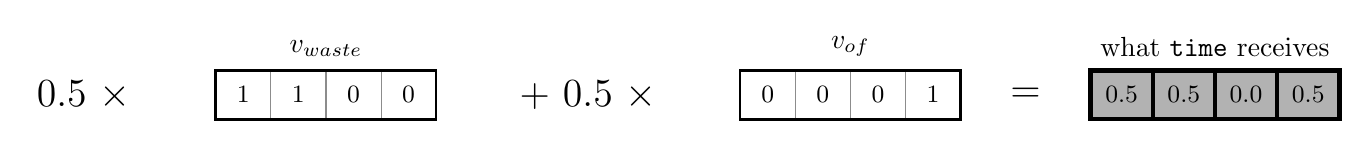
\begin{tikzpicture}
\node[font=\Large] at (1.255,0) {$0.5\ \times$};
\draw[black!45, fill=white] (2.930,0.310) rectangle (3.630,-0.310);
\node[font=\small, text=black] at (3.280,0.000) {$1$};
\draw[black!45, fill=white] (3.630,0.310) rectangle (4.330,-0.310);
\node[font=\small, text=black] at (3.980,0.000) {$1$};
\draw[black!45, fill=white] (4.330,0.310) rectangle (5.030,-0.310);
\node[font=\small, text=black] at (4.680,0.000) {$0$};
\draw[black!45, fill=white] (5.030,0.310) rectangle (5.730,-0.310);
\node[font=\small, text=black] at (5.380,0.000) {$0$};
\draw[line width=0.9pt] (2.930,0.310) rectangle (5.730,-0.310);
\node[anchor=south, font=\normalsize] at (4.330,0.360) {$\bm v_{\text{waste}}$};
\node[font=\Large] at (7.660,0) {$+\ 0.5\ \times$};
\draw[black!45, fill=white] (9.590,0.310) rectangle (10.290,-0.310);
\node[font=\small, text=black] at (9.940,0.000) {$0$};
\draw[black!45, fill=white] (10.290,0.310) rectangle (10.990,-0.310);
\node[font=\small, text=black] at (10.640,0.000) {$0$};
\draw[black!45, fill=white] (10.990,0.310) rectangle (11.690,-0.310);
\node[font=\small, text=black] at (11.340,0.000) {$0$};
\draw[black!45, fill=white] (11.690,0.310) rectangle (12.390,-0.310);
\node[font=\small, text=black] at (12.040,0.000) {$1$};
\draw[line width=0.9pt] (9.590,0.310) rectangle (12.390,-0.310);
\node[anchor=south, font=\normalsize] at (10.990,0.360) {$\bm v_{\text{of}}$};
\node[font=\Large] at (13.215,0) {$=$};
\draw[black!45, fill=black!30] (14.040,0.310) rectangle (14.830,-0.310);
\node[font=\small, text=black] at (14.435,0.000) {$0.5$};
\draw[black!45, fill=black!30] (14.830,0.310) rectangle (15.620,-0.310);
\node[font=\small, text=black] at (15.225,0.000) {$0.5$};
\draw[black!45, fill=black!30] (15.620,0.310) rectangle (16.410,-0.310);
\node[font=\small, text=black] at (16.015,0.000) {$0.0$};
\draw[black!45, fill=black!30] (16.410,0.310) rectangle (17.200,-0.310);
\node[font=\small, text=black] at (16.805,0.000) {$0.5$};
\draw[line width=1.6pt] (14.040,0.310) rectangle (14.830,-0.310);
\draw[line width=1.6pt] (14.830,0.310) rectangle (15.620,-0.310);
\draw[line width=1.6pt] (15.620,0.310) rectangle (16.410,-0.310);
\draw[line width=1.6pt] (16.410,0.310) rectangle (17.200,-0.310);
\draw[line width=0.9pt] (14.040,0.310) rectangle (17.200,-0.310);
\node[anchor=south, font=\normalsize] at (15.620,0.360) {what \texttt{time} receives};
\end{tikzpicture}
\\[10pt]
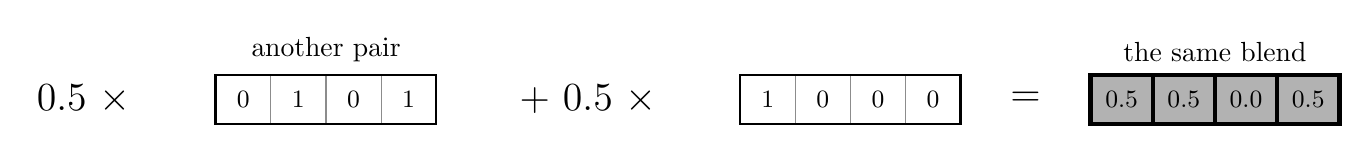
\begin{tikzpicture}
\node[font=\Large] at (1.255,0) {$0.5\ \times$};
\draw[black!45, fill=white] (2.930,0.310) rectangle (3.630,-0.310);
\node[font=\small, text=black] at (3.280,0.000) {$0$};
\draw[black!45, fill=white] (3.630,0.310) rectangle (4.330,-0.310);
\node[font=\small, text=black] at (3.980,0.000) {$1$};
\draw[black!45, fill=white] (4.330,0.310) rectangle (5.030,-0.310);
\node[font=\small, text=black] at (4.680,0.000) {$0$};
\draw[black!45, fill=white] (5.030,0.310) rectangle (5.730,-0.310);
\node[font=\small, text=black] at (5.380,0.000) {$1$};
\draw[line width=0.9pt] (2.930,0.310) rectangle (5.730,-0.310);
\node[anchor=south, font=\normalsize] at (4.330,0.360) {another pair};
\node[font=\Large] at (7.660,0) {$+\ 0.5\ \times$};
\draw[black!45, fill=white] (9.590,0.310) rectangle (10.290,-0.310);
\node[font=\small, text=black] at (9.940,0.000) {$1$};
\draw[black!45, fill=white] (10.290,0.310) rectangle (10.990,-0.310);
\node[font=\small, text=black] at (10.640,0.000) {$0$};
\draw[black!45, fill=white] (10.990,0.310) rectangle (11.690,-0.310);
\node[font=\small, text=black] at (11.340,0.000) {$0$};
\draw[black!45, fill=white] (11.690,0.310) rectangle (12.390,-0.310);
\node[font=\small, text=black] at (12.040,0.000) {$0$};
\draw[line width=0.9pt] (9.590,0.310) rectangle (12.390,-0.310);
\node[anchor=south, font=\normalsize] at (10.990,0.360) {\phantom{p}};
\node[font=\Large] at (13.215,0) {$=$};
\draw[black!45, fill=black!30] (14.040,0.310) rectangle (14.830,-0.310);
\node[font=\small, text=black] at (14.435,0.000) {$0.5$};
\draw[black!45, fill=black!30] (14.830,0.310) rectangle (15.620,-0.310);
\node[font=\small, text=black] at (15.225,0.000) {$0.5$};
\draw[black!45, fill=black!30] (15.620,0.310) rectangle (16.410,-0.310);
\node[font=\small, text=black] at (16.015,0.000) {$0.0$};
\draw[black!45, fill=black!30] (16.410,0.310) rectangle (17.200,-0.310);
\node[font=\small, text=black] at (16.805,0.000) {$0.5$};
\draw[line width=1.6pt] (14.040,0.310) rectangle (14.830,-0.310);
\draw[line width=1.6pt] (14.830,0.310) rectangle (15.620,-0.310);
\draw[line width=1.6pt] (15.620,0.310) rectangle (16.410,-0.310);
\draw[line width=1.6pt] (16.410,0.310) rectangle (17.200,-0.310);
\draw[line width=0.9pt] (14.040,0.310) rectangle (17.200,-0.310);
\node[anchor=south, font=\normalsize] at (15.620,0.360) {the same blend};
\end{tikzpicture}
}
\captionof{figure}{One head, one blend. Top: half of $\bm{v}_{\text{waste}}$ plus half of $\bm{v}_{\text{of}}$, entry by entry. Bottom: a different pair of arrows gives exactly the same shaded result, so the result alone cannot say who said what.}
\label{fig:ch5blend}
\end{center}
 Two different pairs of reports, one identical blend: after the
averaging, the token cannot know which pair it heard. A weighted average is a single arrow, and a single
arrow can be built from many different mixtures.

\begin{breaks}
The microphone picture suggests the information is gone for good. In a trained model the value arrows are
learned, and they can be made to point in separate directions so that a blend is still readable. The real
limit is that one head has one set of shares: it must decide how much \tok{waste} matters and how much
\tok{of} matters with a single softmax, so emphasising one always takes attention from the other.
\end{breaks}

\Why A softmax hands out shares that add to 1. So within one head, attention is a fixed budget, and every
question competes for it. To ask two questions without competition, you need two budgets.

\begin{wrongidea}{5.2}
\emph{One head can attend to two tokens equally well, by giving each 50\%.} It can attend to both, but it
cannot keep their messages apart, and it cannot make one share bigger without shrinking the other. That is
the difference between ``listening to two people'' and ``hearing two people talk at once''.
\end{wrongidea}

\begin{checkq}
A single head gives \tok{time} the shares $(0.5, 0.5, 0)$ over \tok{waste}, \tok{of}, \tok{time}. What can
\tok{time} tell from the output alone?
\begin{options}
\item Exactly what \tok{waste} said and exactly what \tok{of} said.
\item The average of what they said, but not which part came from whom.
\item Nothing at all, because averages destroy everything.
\item What \tok{time} itself said, since it always attends to itself.
\end{options}
\end{checkq}

\Summary{One head returns one weighted average, so asking two questions needs two heads.}

%---------------------------------------------------------------------
\subsection*{5.2\quad Two heads, each half as wide}

\Picture Instead of one reporter who listens to everyone, send two reporters with different briefs. One is
told ``find any judgement nearby''. The other is told ``find the small linking words''. Each writes a short
note.

The budget does not grow. Our arrows still have $d=4$ numbers, so the two heads get $d_k=2$ each. In the
same way, a model with width 64 and two heads gives each head 32 recipes. Each head is narrower, and in exchange there are more of them.

\paragraph{Worked example: head 1, fully.} Head 1 has its own three machines, each $4\times2$ (four
numbers in, two out):
\[
W_Q^{(1)}=\nFiveWQone,\quad W_K^{(1)}=\nFiveWKone,\quad W_V^{(1)}=\nFiveWVone \shape{d\times d_k=4\times2}
\]
Figure~\ref{fig:ch5headone} does the three products. In each one, the outlined row meets the outlined
column, and the dark cell is the number they make.

\begin{center}
\fitwidthFourFive{% AUTO-GENERATED by code/figlib.py helpers -- do not edit
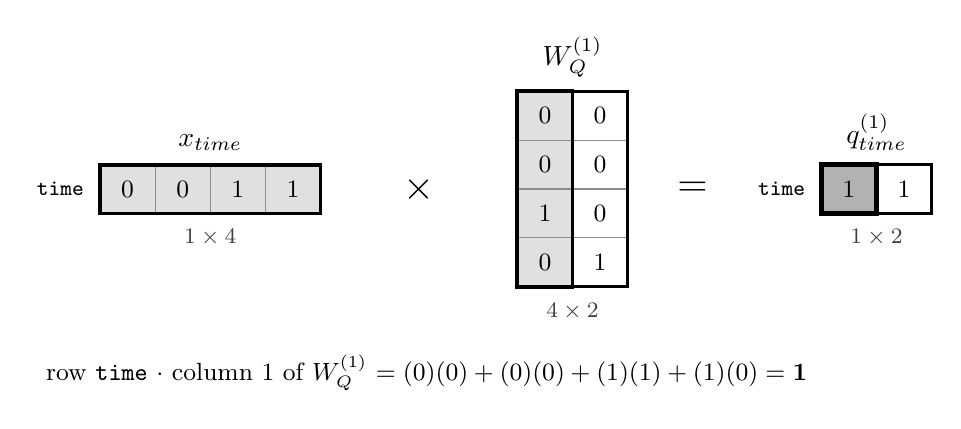
\begin{tikzpicture}
\draw[black!45, fill=black!12] (0.810,0.310) rectangle (1.510,-0.310);
\node[font=\small, text=black] at (1.160,0.000) {$0$};
\draw[black!45, fill=black!12] (1.510,0.310) rectangle (2.210,-0.310);
\node[font=\small, text=black] at (1.860,0.000) {$0$};
\draw[black!45, fill=black!12] (2.210,0.310) rectangle (2.910,-0.310);
\node[font=\small, text=black] at (2.560,0.000) {$1$};
\draw[black!45, fill=black!12] (2.910,0.310) rectangle (3.610,-0.310);
\node[font=\small, text=black] at (3.260,0.000) {$1$};
\draw[line width=1.4pt] (0.810,0.310) rectangle (3.610,-0.310);
\draw[line width=0.9pt] (0.810,0.310) rectangle (3.610,-0.310);
\node[anchor=east, font=\footnotesize\ttfamily] at (0.730,0.000) {time};
\node[anchor=south, font=\normalsize] at (2.210,0.360) {$\bm x_{\text{time}}$};
\node[anchor=north, font=\footnotesize, text=black!75] at (2.210,-0.390) {$1\times4$};
\node[font=\Large] at (4.860,0) {$\times$};
\draw[black!45, fill=black!12] (6.110,1.240) rectangle (6.810,0.620);
\node[font=\small, text=black] at (6.460,0.930) {$0$};
\draw[black!45, fill=white] (6.810,1.240) rectangle (7.510,0.620);
\node[font=\small, text=black] at (7.160,0.930) {$0$};
\draw[black!45, fill=black!12] (6.110,0.620) rectangle (6.810,0.000);
\node[font=\small, text=black] at (6.460,0.310) {$0$};
\draw[black!45, fill=white] (6.810,0.620) rectangle (7.510,0.000);
\node[font=\small, text=black] at (7.160,0.310) {$0$};
\draw[black!45, fill=black!12] (6.110,0.000) rectangle (6.810,-0.620);
\node[font=\small, text=black] at (6.460,-0.310) {$1$};
\draw[black!45, fill=white] (6.810,0.000) rectangle (7.510,-0.620);
\node[font=\small, text=black] at (7.160,-0.310) {$0$};
\draw[black!45, fill=black!12] (6.110,-0.620) rectangle (6.810,-1.240);
\node[font=\small, text=black] at (6.460,-0.930) {$0$};
\draw[black!45, fill=white] (6.810,-0.620) rectangle (7.510,-1.240);
\node[font=\small, text=black] at (7.160,-0.930) {$1$};
\draw[line width=1.4pt] (6.110,1.240) rectangle (6.810,-1.240);
\draw[line width=0.9pt] (6.110,1.240) rectangle (7.510,-1.240);
\node[anchor=south, font=\normalsize] at (6.810,1.290) {$W_Q^{(1)}$};
\node[anchor=north, font=\footnotesize, text=black!75] at (6.810,-1.320) {$4\times2$};
\node[font=\Large] at (8.335,0) {$=$};
\draw[black!45, fill=black!30] (9.970,0.310) rectangle (10.670,-0.310);
\node[font=\small, text=black] at (10.320,0.000) {$1$};
\draw[black!45, fill=white] (10.670,0.310) rectangle (11.370,-0.310);
\node[font=\small, text=black] at (11.020,0.000) {$1$};
\draw[line width=1.6pt] (9.970,0.310) rectangle (10.670,-0.310);
\draw[line width=0.9pt] (9.970,0.310) rectangle (11.370,-0.310);
\node[anchor=east, font=\footnotesize\ttfamily] at (9.890,0.000) {time};
\node[anchor=south, font=\normalsize] at (10.670,0.360) {$\bm q^{(1)}_{\text{time}}$};
\node[anchor=north, font=\footnotesize, text=black!75] at (10.670,-0.390) {$1\times2$};
\node[anchor=north west, font=\small, align=left] at (0,-1.990) {row \texttt{time} $\cdot$ column 1 of $W_Q^{(1)}$ $= (0)(0) + (0)(0) + (1)(1) + (1)(0) = \mathbf{1}$};
\end{tikzpicture}
\\[10pt]
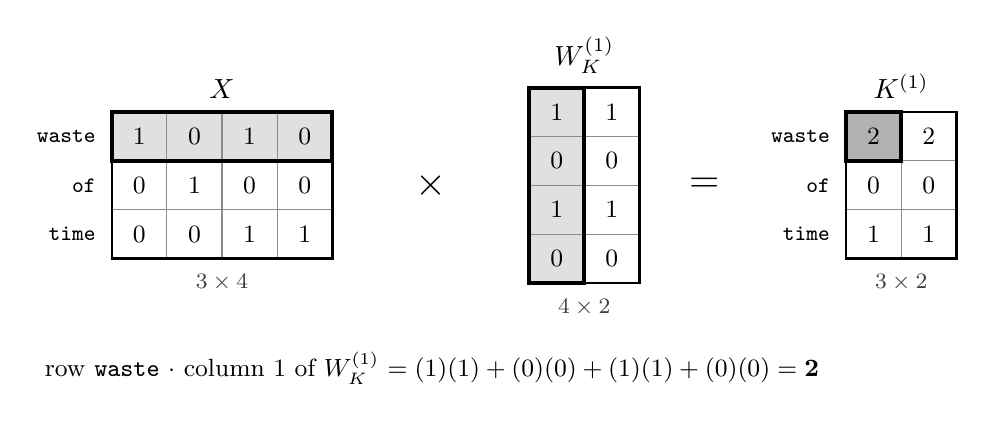
\begin{tikzpicture}
\draw[black!45, fill=black!12] (0.975,0.930) rectangle (1.675,0.310);
\node[font=\small, text=black] at (1.325,0.620) {$1$};
\draw[black!45, fill=black!12] (1.675,0.930) rectangle (2.375,0.310);
\node[font=\small, text=black] at (2.025,0.620) {$0$};
\draw[black!45, fill=black!12] (2.375,0.930) rectangle (3.075,0.310);
\node[font=\small, text=black] at (2.725,0.620) {$1$};
\draw[black!45, fill=black!12] (3.075,0.930) rectangle (3.775,0.310);
\node[font=\small, text=black] at (3.425,0.620) {$0$};
\draw[black!45, fill=white] (0.975,0.310) rectangle (1.675,-0.310);
\node[font=\small, text=black] at (1.325,-0.000) {$0$};
\draw[black!45, fill=white] (1.675,0.310) rectangle (2.375,-0.310);
\node[font=\small, text=black] at (2.025,-0.000) {$1$};
\draw[black!45, fill=white] (2.375,0.310) rectangle (3.075,-0.310);
\node[font=\small, text=black] at (2.725,-0.000) {$0$};
\draw[black!45, fill=white] (3.075,0.310) rectangle (3.775,-0.310);
\node[font=\small, text=black] at (3.425,-0.000) {$0$};
\draw[black!45, fill=white] (0.975,-0.310) rectangle (1.675,-0.930);
\node[font=\small, text=black] at (1.325,-0.620) {$0$};
\draw[black!45, fill=white] (1.675,-0.310) rectangle (2.375,-0.930);
\node[font=\small, text=black] at (2.025,-0.620) {$0$};
\draw[black!45, fill=white] (2.375,-0.310) rectangle (3.075,-0.930);
\node[font=\small, text=black] at (2.725,-0.620) {$1$};
\draw[black!45, fill=white] (3.075,-0.310) rectangle (3.775,-0.930);
\node[font=\small, text=black] at (3.425,-0.620) {$1$};
\draw[line width=1.4pt] (0.975,0.930) rectangle (3.775,0.310);
\draw[line width=0.9pt] (0.975,0.930) rectangle (3.775,-0.930);
\node[anchor=east, font=\footnotesize\ttfamily] at (0.895,0.620) {waste};
\node[anchor=east, font=\footnotesize\ttfamily] at (0.895,-0.000) {of};
\node[anchor=east, font=\footnotesize\ttfamily] at (0.895,-0.620) {time};
\node[anchor=south, font=\normalsize] at (2.375,0.980) {$X$};
\node[anchor=north, font=\footnotesize, text=black!75] at (2.375,-1.010) {$3\times4$};
\node[font=\Large] at (5.025,0) {$\times$};
\draw[black!45, fill=black!12] (6.275,1.240) rectangle (6.975,0.620);
\node[font=\small, text=black] at (6.625,0.930) {$1$};
\draw[black!45, fill=white] (6.975,1.240) rectangle (7.675,0.620);
\node[font=\small, text=black] at (7.325,0.930) {$1$};
\draw[black!45, fill=black!12] (6.275,0.620) rectangle (6.975,0.000);
\node[font=\small, text=black] at (6.625,0.310) {$0$};
\draw[black!45, fill=white] (6.975,0.620) rectangle (7.675,0.000);
\node[font=\small, text=black] at (7.325,0.310) {$0$};
\draw[black!45, fill=black!12] (6.275,0.000) rectangle (6.975,-0.620);
\node[font=\small, text=black] at (6.625,-0.310) {$1$};
\draw[black!45, fill=white] (6.975,0.000) rectangle (7.675,-0.620);
\node[font=\small, text=black] at (7.325,-0.310) {$1$};
\draw[black!45, fill=black!12] (6.275,-0.620) rectangle (6.975,-1.240);
\node[font=\small, text=black] at (6.625,-0.930) {$0$};
\draw[black!45, fill=white] (6.975,-0.620) rectangle (7.675,-1.240);
\node[font=\small, text=black] at (7.325,-0.930) {$0$};
\draw[line width=1.4pt] (6.275,1.240) rectangle (6.975,-1.240);
\draw[line width=0.9pt] (6.275,1.240) rectangle (7.675,-1.240);
\node[anchor=south, font=\normalsize] at (6.975,1.290) {$W_K^{(1)}$};
\node[anchor=north, font=\footnotesize, text=black!75] at (6.975,-1.320) {$4\times2$};
\node[font=\Large] at (8.500,0) {$=$};
\draw[black!45, fill=black!30] (10.300,0.930) rectangle (11.000,0.310);
\node[font=\small, text=black] at (10.650,0.620) {$2$};
\draw[black!45, fill=white] (11.000,0.930) rectangle (11.700,0.310);
\node[font=\small, text=black] at (11.350,0.620) {$2$};
\draw[black!45, fill=white] (10.300,0.310) rectangle (11.000,-0.310);
\node[font=\small, text=black] at (10.650,-0.000) {$0$};
\draw[black!45, fill=white] (11.000,0.310) rectangle (11.700,-0.310);
\node[font=\small, text=black] at (11.350,-0.000) {$0$};
\draw[black!45, fill=white] (10.300,-0.310) rectangle (11.000,-0.930);
\node[font=\small, text=black] at (10.650,-0.620) {$1$};
\draw[black!45, fill=white] (11.000,-0.310) rectangle (11.700,-0.930);
\node[font=\small, text=black] at (11.350,-0.620) {$1$};
\draw[line width=1.6pt] (10.300,0.930) rectangle (11.000,0.310);
\draw[line width=0.9pt] (10.300,0.930) rectangle (11.700,-0.930);
\node[anchor=east, font=\footnotesize\ttfamily] at (10.220,0.620) {waste};
\node[anchor=east, font=\footnotesize\ttfamily] at (10.220,-0.000) {of};
\node[anchor=east, font=\footnotesize\ttfamily] at (10.220,-0.620) {time};
\node[anchor=south, font=\normalsize] at (11.000,0.980) {$K^{(1)}$};
\node[anchor=north, font=\footnotesize, text=black!75] at (11.000,-1.010) {$3\times2$};
\node[anchor=north west, font=\small, align=left] at (0,-1.990) {row \texttt{waste} $\cdot$ column 1 of $W_K^{(1)}$ $= (1)(1) + (0)(0) + (1)(1) + (0)(0) = \mathbf{2}$};
\end{tikzpicture}
\\[10pt]
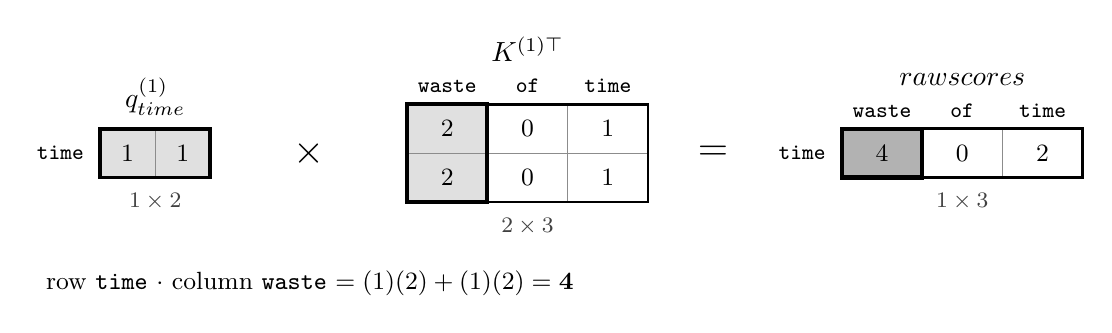
\begin{tikzpicture}
\draw[black!45, fill=black!12] (0.810,0.310) rectangle (1.510,-0.310);
\node[font=\small, text=black] at (1.160,0.000) {$1$};
\draw[black!45, fill=black!12] (1.510,0.310) rectangle (2.210,-0.310);
\node[font=\small, text=black] at (1.860,0.000) {$1$};
\draw[line width=1.4pt] (0.810,0.310) rectangle (2.210,-0.310);
\draw[line width=0.9pt] (0.810,0.310) rectangle (2.210,-0.310);
\node[anchor=east, font=\footnotesize\ttfamily] at (0.730,0.000) {time};
\node[anchor=south, font=\normalsize] at (1.510,0.360) {$\bm q^{(1)}_{\text{time}}$};
\node[anchor=north, font=\footnotesize, text=black!75] at (1.510,-0.390) {$1\times2$};
\node[font=\Large] at (3.460,0) {$\times$};
\draw[black!45, fill=black!12] (4.710,0.620) rectangle (5.730,0.000);
\node[font=\small, text=black] at (5.220,0.310) {$2$};
\draw[black!45, fill=white] (5.730,0.620) rectangle (6.750,0.000);
\node[font=\small, text=black] at (6.240,0.310) {$0$};
\draw[black!45, fill=white] (6.750,0.620) rectangle (7.770,0.000);
\node[font=\small, text=black] at (7.260,0.310) {$1$};
\draw[black!45, fill=black!12] (4.710,0.000) rectangle (5.730,-0.620);
\node[font=\small, text=black] at (5.220,-0.310) {$2$};
\draw[black!45, fill=white] (5.730,0.000) rectangle (6.750,-0.620);
\node[font=\small, text=black] at (6.240,-0.310) {$0$};
\draw[black!45, fill=white] (6.750,0.000) rectangle (7.770,-0.620);
\node[font=\small, text=black] at (7.260,-0.310) {$1$};
\draw[line width=1.4pt] (4.710,0.620) rectangle (5.730,-0.620);
\draw[line width=0.9pt] (4.710,0.620) rectangle (7.770,-0.620);
\node[anchor=south, font=\footnotesize\ttfamily] at (5.220,0.640) {waste};
\node[anchor=south, font=\footnotesize\ttfamily] at (6.240,0.640) {of};
\node[anchor=south, font=\footnotesize\ttfamily] at (7.260,0.640) {time};
\node[anchor=south, font=\normalsize] at (6.240,1.040) {$K^{(1)\top}$};
\node[anchor=north, font=\footnotesize, text=black!75] at (6.240,-0.700) {$2\times3$};
\node[font=\Large] at (8.595,0) {$=$};
\draw[black!45, fill=black!30] (10.230,0.310) rectangle (11.250,-0.310);
\node[font=\small, text=black] at (10.740,0.000) {$4$};
\draw[black!45, fill=white] (11.250,0.310) rectangle (12.270,-0.310);
\node[font=\small, text=black] at (11.760,0.000) {$0$};
\draw[black!45, fill=white] (12.270,0.310) rectangle (13.290,-0.310);
\node[font=\small, text=black] at (12.780,0.000) {$2$};
\draw[line width=1.6pt] (10.230,0.310) rectangle (11.250,-0.310);
\draw[line width=0.9pt] (10.230,0.310) rectangle (13.290,-0.310);
\node[anchor=east, font=\footnotesize\ttfamily] at (10.150,0.000) {time};
\node[anchor=south, font=\footnotesize\ttfamily] at (10.740,0.330) {waste};
\node[anchor=south, font=\footnotesize\ttfamily] at (11.760,0.330) {of};
\node[anchor=south, font=\footnotesize\ttfamily] at (12.780,0.330) {time};
\node[anchor=south, font=\normalsize] at (11.760,0.730) {$\text{raw scores}$};
\node[anchor=north, font=\footnotesize, text=black!75] at (11.760,-0.390) {$1\times3$};
\node[anchor=north west, font=\small, align=left] at (0,-1.370) {row \texttt{time} $\cdot$ column \texttt{waste} $= (1)(2) + (1)(2) = \mathbf{4}$};
\end{tikzpicture}
}
\captionof{figure}{Head 1, step by step. Top: \tok{time}'s arrow through $W_Q^{(1)}$ gives its $1\times2$ query. Middle: every token's arrow through $W_K^{(1)}$ gives one key per row. Bottom: the query against the transposed keys gives one raw score per token; \tok{waste} wins with 4.}
\label{fig:ch5headone}
\end{center}

So the raw scores are $\nFiveSone$. Dividing by $\sqrt{d_k}=\sqrt2$ gives $\nFiveSoneScaled$, and the softmax gives the shares
\[
\bm{a}^{(1)}_{\text{time}} = (\nFiveAoneWaste,\ \nFiveAoneOf,\ \nFiveAoneTime).
\]
Head 1 gives \nFivePoneWaste\% of its attention to \tok{waste}. It is the judgement-finder.

\paragraph{Head 2: your turn.} Head 2 uses
\[
W_Q^{(2)}=\nFiveWQtwo,\quad W_K^{(2)}=\nFiveWKtwo .
\]
\Predict Look at the second row of $W_K^{(2)}$: only \tok{of}, whose arrow is $(0,1,0,0)$, can produce a
non-zero key. Which token will head 2 favour? Fill in the question marks of Figure~\ref{fig:ch5headtwo}:
$\bm{q}^{(2)}_{\text{time}}$, the three keys, then the three raw scores. Check with Answer 5.2.

\begin{center}
\fitwidthFourFive{% AUTO-GENERATED by code/figlib.py helpers -- do not edit
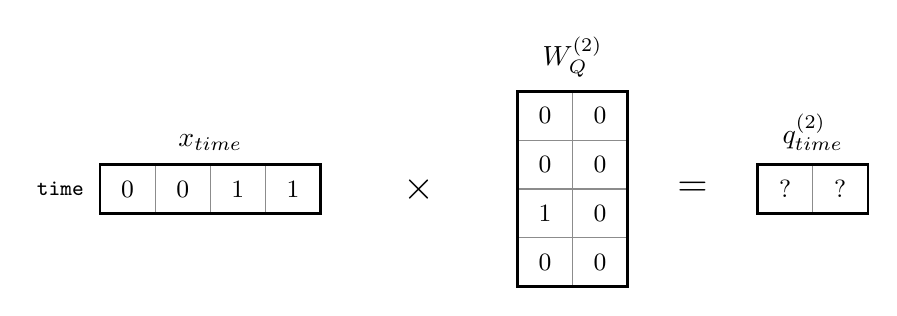
\begin{tikzpicture}
\draw[black!45, fill=white] (0.810,0.310) rectangle (1.510,-0.310);
\node[font=\small, text=black] at (1.160,0.000) {$0$};
\draw[black!45, fill=white] (1.510,0.310) rectangle (2.210,-0.310);
\node[font=\small, text=black] at (1.860,0.000) {$0$};
\draw[black!45, fill=white] (2.210,0.310) rectangle (2.910,-0.310);
\node[font=\small, text=black] at (2.560,0.000) {$1$};
\draw[black!45, fill=white] (2.910,0.310) rectangle (3.610,-0.310);
\node[font=\small, text=black] at (3.260,0.000) {$1$};
\draw[line width=0.9pt] (0.810,0.310) rectangle (3.610,-0.310);
\node[anchor=east, font=\footnotesize\ttfamily] at (0.730,0.000) {time};
\node[anchor=south, font=\normalsize] at (2.210,0.360) {$\bm x_{\text{time}}$};
\node[font=\Large] at (4.860,0) {$\times$};
\draw[black!45, fill=white] (6.110,1.240) rectangle (6.810,0.620);
\node[font=\small, text=black] at (6.460,0.930) {$0$};
\draw[black!45, fill=white] (6.810,1.240) rectangle (7.510,0.620);
\node[font=\small, text=black] at (7.160,0.930) {$0$};
\draw[black!45, fill=white] (6.110,0.620) rectangle (6.810,0.000);
\node[font=\small, text=black] at (6.460,0.310) {$0$};
\draw[black!45, fill=white] (6.810,0.620) rectangle (7.510,0.000);
\node[font=\small, text=black] at (7.160,0.310) {$0$};
\draw[black!45, fill=white] (6.110,0.000) rectangle (6.810,-0.620);
\node[font=\small, text=black] at (6.460,-0.310) {$1$};
\draw[black!45, fill=white] (6.810,0.000) rectangle (7.510,-0.620);
\node[font=\small, text=black] at (7.160,-0.310) {$0$};
\draw[black!45, fill=white] (6.110,-0.620) rectangle (6.810,-1.240);
\node[font=\small, text=black] at (6.460,-0.930) {$0$};
\draw[black!45, fill=white] (6.810,-0.620) rectangle (7.510,-1.240);
\node[font=\small, text=black] at (7.160,-0.930) {$0$};
\draw[line width=0.9pt] (6.110,1.240) rectangle (7.510,-1.240);
\node[anchor=south, font=\normalsize] at (6.810,1.290) {$W_Q^{(2)}$};
\node[font=\Large] at (8.335,0) {$=$};
\draw[black!45, fill=white] (9.160,0.310) rectangle (9.860,-0.310);
\node[font=\small, text=black] at (9.510,0.000) {?};
\draw[black!45, fill=white] (9.860,0.310) rectangle (10.560,-0.310);
\node[font=\small, text=black] at (10.210,0.000) {?};
\draw[line width=0.9pt] (9.160,0.310) rectangle (10.560,-0.310);
\node[anchor=south, font=\normalsize] at (9.860,0.360) {$\bm q^{(2)}_{\text{time}}$};
\end{tikzpicture}
\\[10pt]
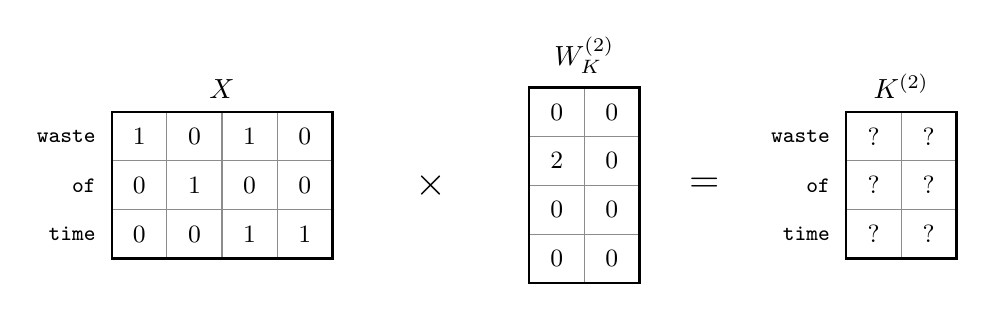
\begin{tikzpicture}
\draw[black!45, fill=white] (0.975,0.930) rectangle (1.675,0.310);
\node[font=\small, text=black] at (1.325,0.620) {$1$};
\draw[black!45, fill=white] (1.675,0.930) rectangle (2.375,0.310);
\node[font=\small, text=black] at (2.025,0.620) {$0$};
\draw[black!45, fill=white] (2.375,0.930) rectangle (3.075,0.310);
\node[font=\small, text=black] at (2.725,0.620) {$1$};
\draw[black!45, fill=white] (3.075,0.930) rectangle (3.775,0.310);
\node[font=\small, text=black] at (3.425,0.620) {$0$};
\draw[black!45, fill=white] (0.975,0.310) rectangle (1.675,-0.310);
\node[font=\small, text=black] at (1.325,-0.000) {$0$};
\draw[black!45, fill=white] (1.675,0.310) rectangle (2.375,-0.310);
\node[font=\small, text=black] at (2.025,-0.000) {$1$};
\draw[black!45, fill=white] (2.375,0.310) rectangle (3.075,-0.310);
\node[font=\small, text=black] at (2.725,-0.000) {$0$};
\draw[black!45, fill=white] (3.075,0.310) rectangle (3.775,-0.310);
\node[font=\small, text=black] at (3.425,-0.000) {$0$};
\draw[black!45, fill=white] (0.975,-0.310) rectangle (1.675,-0.930);
\node[font=\small, text=black] at (1.325,-0.620) {$0$};
\draw[black!45, fill=white] (1.675,-0.310) rectangle (2.375,-0.930);
\node[font=\small, text=black] at (2.025,-0.620) {$0$};
\draw[black!45, fill=white] (2.375,-0.310) rectangle (3.075,-0.930);
\node[font=\small, text=black] at (2.725,-0.620) {$1$};
\draw[black!45, fill=white] (3.075,-0.310) rectangle (3.775,-0.930);
\node[font=\small, text=black] at (3.425,-0.620) {$1$};
\draw[line width=0.9pt] (0.975,0.930) rectangle (3.775,-0.930);
\node[anchor=east, font=\footnotesize\ttfamily] at (0.895,0.620) {waste};
\node[anchor=east, font=\footnotesize\ttfamily] at (0.895,-0.000) {of};
\node[anchor=east, font=\footnotesize\ttfamily] at (0.895,-0.620) {time};
\node[anchor=south, font=\normalsize] at (2.375,0.980) {$X$};
\node[font=\Large] at (5.025,0) {$\times$};
\draw[black!45, fill=white] (6.275,1.240) rectangle (6.975,0.620);
\node[font=\small, text=black] at (6.625,0.930) {$0$};
\draw[black!45, fill=white] (6.975,1.240) rectangle (7.675,0.620);
\node[font=\small, text=black] at (7.325,0.930) {$0$};
\draw[black!45, fill=white] (6.275,0.620) rectangle (6.975,0.000);
\node[font=\small, text=black] at (6.625,0.310) {$2$};
\draw[black!45, fill=white] (6.975,0.620) rectangle (7.675,0.000);
\node[font=\small, text=black] at (7.325,0.310) {$0$};
\draw[black!45, fill=white] (6.275,0.000) rectangle (6.975,-0.620);
\node[font=\small, text=black] at (6.625,-0.310) {$0$};
\draw[black!45, fill=white] (6.975,0.000) rectangle (7.675,-0.620);
\node[font=\small, text=black] at (7.325,-0.310) {$0$};
\draw[black!45, fill=white] (6.275,-0.620) rectangle (6.975,-1.240);
\node[font=\small, text=black] at (6.625,-0.930) {$0$};
\draw[black!45, fill=white] (6.975,-0.620) rectangle (7.675,-1.240);
\node[font=\small, text=black] at (7.325,-0.930) {$0$};
\draw[line width=0.9pt] (6.275,1.240) rectangle (7.675,-1.240);
\node[anchor=south, font=\normalsize] at (6.975,1.290) {$W_K^{(2)}$};
\node[font=\Large] at (8.500,0) {$=$};
\draw[black!45, fill=white] (10.300,0.930) rectangle (11.000,0.310);
\node[font=\small, text=black] at (10.650,0.620) {?};
\draw[black!45, fill=white] (11.000,0.930) rectangle (11.700,0.310);
\node[font=\small, text=black] at (11.350,0.620) {?};
\draw[black!45, fill=white] (10.300,0.310) rectangle (11.000,-0.310);
\node[font=\small, text=black] at (10.650,-0.000) {?};
\draw[black!45, fill=white] (11.000,0.310) rectangle (11.700,-0.310);
\node[font=\small, text=black] at (11.350,-0.000) {?};
\draw[black!45, fill=white] (10.300,-0.310) rectangle (11.000,-0.930);
\node[font=\small, text=black] at (10.650,-0.620) {?};
\draw[black!45, fill=white] (11.000,-0.310) rectangle (11.700,-0.930);
\node[font=\small, text=black] at (11.350,-0.620) {?};
\draw[line width=0.9pt] (10.300,0.930) rectangle (11.700,-0.930);
\node[anchor=east, font=\footnotesize\ttfamily] at (10.220,0.620) {waste};
\node[anchor=east, font=\footnotesize\ttfamily] at (10.220,-0.000) {of};
\node[anchor=east, font=\footnotesize\ttfamily] at (10.220,-0.620) {time};
\node[anchor=south, font=\normalsize] at (11.000,0.980) {$K^{(2)}$};
\end{tikzpicture}
}
\captionof{figure}{Head 2, your turn. Multiply as in Figure~\ref{fig:ch5headone} and fill in the cells marked ?.}
\label{fig:ch5headtwo}
\end{center}


\Sanity The scaled scores are
\[\nFiveStwoScaled,\]
and the shares come out as $(\nFiveAtwoWaste,\ \nFiveAtwoOf,\ \nFiveAtwoTime)$: \nFivePtwoOf\% on \tok{of}. The shares add to 1, and the
favourite is the token you predicted.

\begin{center}
\small
\begin{tabular}{@{}l c c c@{}}
\toprule
\tok{time} attends to & \tok{waste} & \tok{of} & \tok{time}\\
\midrule
Chapter 3 (one head, $d_k=4$) & \nFiveChThreeWaste\% & \nFiveChThreeOf\% & \apctTime\%\\
Head 1 ($d_k=2$) & \nFivePoneWaste\% & \nFivePoneOf\% & \nFivePoneTime\%\\
Head 2 ($d_k=2$) & \nFivePtwoWaste\% & \nFivePtwoOf\% & \nFivePtwoTime\%\\
\bottomrule
\end{tabular}
\end{center}

Each head now spends its whole budget on its own question. One head mostly hears \tok{waste}; the other mostly
hears \tok{of}.

\begin{breaks}
Our two reporters have tidy, nameable briefs because we wrote the weights by hand. Heads in trained models
are learned, often overlap, and many have no neat job. Michel, Levy and Neubig (2019) removed most of the heads
of trained models one at a time and found that many could go with little loss.
\end{breaks}

\Why Splitting the width keeps the cost the same (the four machines of the block still hold $4\times d^2$
numbers in total) while giving the token several independent budgets of attention. The price is that each head
asks with fewer numbers, so each question is cruder.

\begin{wrongidea}{5.1}
\emph{More heads is always better.} With the width fixed, more heads means narrower heads. Taken to the
extreme, a head with $d_k=1$ compares single numbers, a very blunt question. The number of heads is a trade-off to choose, and Chapter 11
treats it as one.
\end{wrongidea}

\begin{wrongidea}{5.5}
\emph{Each head has a fixed job, like ``the grammar head''.} Our toy heads do, because we designed them. In a
trained model a head's job is whatever helped predict the next token, and it is often a mixture.
\end{wrongidea}

\begin{checkq}
A model has width $d=64$. You change it from 2 heads to 8 heads and keep $d$ fixed. What happens?
\begin{options}
\item Each head becomes 4 times wider, so each question is sharper.
\item Each head drops from 32 to 8 numbers, and there are 4 times as many independent sets of shares.
\item The number of attention weights grows 4 times.
\item The model necessarily gets better, because more heads see more.
\end{options}
\end{checkq}

\Summary{Splitting the width into heads gives a token several separate attention budgets at no extra cost,
each one asking a cruder question.}

%---------------------------------------------------------------------
\subsection*{5.3\quad Stitching the notes together}

\Picture The two reporters staple their notes side by side, and an editor rewrites the stapled page in the
house style.

\Exactly Each head hands back a short arrow for \tok{time}, of width $d_k=2$. Concatenate them into one
arrow of width $d=4$, then multiply by an output matrix $W_O$ ($d\times d$), the editor:
\[
\bm{o}_{\text{time}} = \big[\,\bm{o}^{(1)}_{\text{time}}\ \ \bm{o}^{(2)}_{\text{time}}\,\big]\,W_O \shape{(1\times d)(d\times d)=1\times d}
\]
Figure~\ref{fig:ch5concat} shows both steps with the numbers.

\begin{center}
\fitwidthFourFive{% AUTO-GENERATED by code/figlib.py helpers -- do not edit
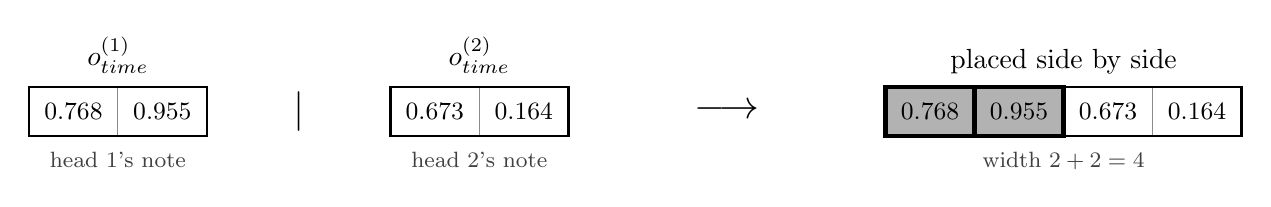
\begin{tikzpicture}
\draw[black!45, fill=white] (0.000,0.310) rectangle (1.130,-0.310);
\node[font=\small, text=black] at (0.565,0.000) {$0.768$};
\draw[black!45, fill=white] (1.130,0.310) rectangle (2.260,-0.310);
\node[font=\small, text=black] at (1.695,0.000) {$0.955$};
\draw[line width=0.9pt] (0.000,0.310) rectangle (2.260,-0.310);
\node[anchor=south, font=\normalsize] at (1.130,0.360) {$\bm o^{(1)}_{\text{time}}$};
\node[anchor=north, font=\footnotesize, text=black!75] at (1.130,-0.390) {head 1's note};
\node[font=\Large] at (3.425,0) {$\big|$};
\draw[black!45, fill=white] (4.590,0.310) rectangle (5.720,-0.310);
\node[font=\small, text=black] at (5.155,0.000) {$0.673$};
\draw[black!45, fill=white] (5.720,0.310) rectangle (6.850,-0.310);
\node[font=\small, text=black] at (6.285,0.000) {$0.164$};
\draw[line width=0.9pt] (4.590,0.310) rectangle (6.850,-0.310);
\node[anchor=south, font=\normalsize] at (5.720,0.360) {$\bm o^{(2)}_{\text{time}}$};
\node[anchor=north, font=\footnotesize, text=black!75] at (5.720,-0.390) {head 2's note};
\node[font=\Large] at (8.865,0) {$\longrightarrow$};
\draw[black!45, fill=black!30] (10.880,0.310) rectangle (12.010,-0.310);
\node[font=\small, text=black] at (11.445,0.000) {$0.768$};
\draw[black!45, fill=black!30] (12.010,0.310) rectangle (13.140,-0.310);
\node[font=\small, text=black] at (12.575,0.000) {$0.955$};
\draw[black!45, fill=white] (13.140,0.310) rectangle (14.270,-0.310);
\node[font=\small, text=black] at (13.705,0.000) {$0.673$};
\draw[black!45, fill=white] (14.270,0.310) rectangle (15.400,-0.310);
\node[font=\small, text=black] at (14.835,0.000) {$0.164$};
\draw[line width=1.6pt] (10.880,0.310) rectangle (12.010,-0.310);
\draw[line width=1.6pt] (12.010,0.310) rectangle (13.140,-0.310);
\draw[line width=0.9pt] (10.880,0.310) rectangle (15.400,-0.310);
\node[anchor=south, font=\normalsize] at (13.140,0.360) {placed side by side};
\node[anchor=north, font=\footnotesize, text=black!75] at (13.140,-0.390) {width $2+2=4$};
\end{tikzpicture}
\\[10pt]
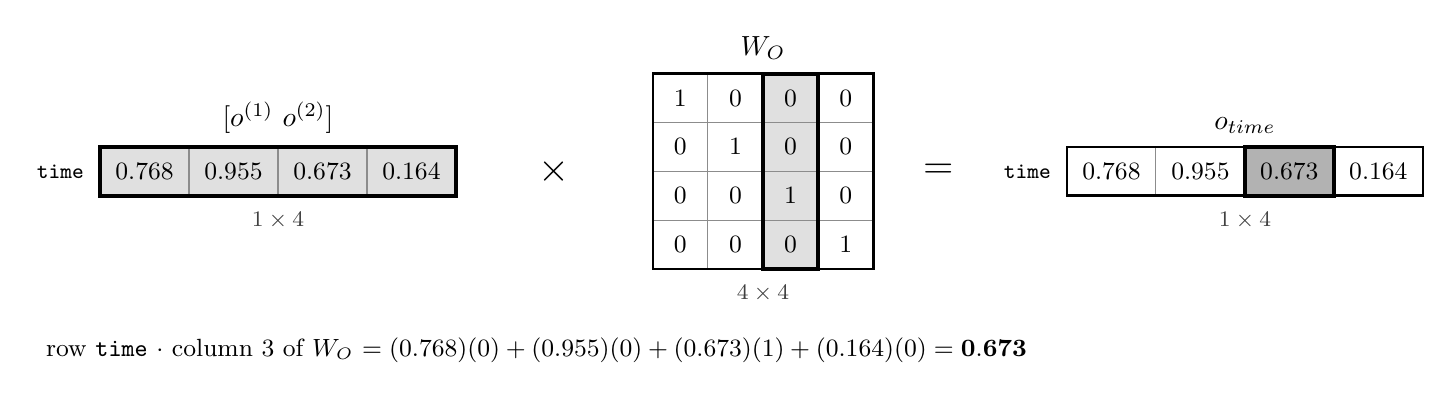
\begin{tikzpicture}
\draw[black!45, fill=black!12] (0.810,0.310) rectangle (1.940,-0.310);
\node[font=\small, text=black] at (1.375,0.000) {$0.768$};
\draw[black!45, fill=black!12] (1.940,0.310) rectangle (3.070,-0.310);
\node[font=\small, text=black] at (2.505,0.000) {$0.955$};
\draw[black!45, fill=black!12] (3.070,0.310) rectangle (4.200,-0.310);
\node[font=\small, text=black] at (3.635,0.000) {$0.673$};
\draw[black!45, fill=black!12] (4.200,0.310) rectangle (5.330,-0.310);
\node[font=\small, text=black] at (4.765,0.000) {$0.164$};
\draw[line width=1.4pt] (0.810,0.310) rectangle (5.330,-0.310);
\draw[line width=0.9pt] (0.810,0.310) rectangle (5.330,-0.310);
\node[anchor=east, font=\footnotesize\ttfamily] at (0.730,0.000) {time};
\node[anchor=south, font=\normalsize] at (3.070,0.360) {$[\bm o^{(1)}\ \bm o^{(2)}]$};
\node[anchor=north, font=\footnotesize, text=black!75] at (3.070,-0.390) {$1\times4$};
\node[font=\Large] at (6.580,0) {$\times$};
\draw[black!45, fill=white] (7.830,1.240) rectangle (8.530,0.620);
\node[font=\small, text=black] at (8.180,0.930) {$1$};
\draw[black!45, fill=white] (8.530,1.240) rectangle (9.230,0.620);
\node[font=\small, text=black] at (8.880,0.930) {$0$};
\draw[black!45, fill=black!12] (9.230,1.240) rectangle (9.930,0.620);
\node[font=\small, text=black] at (9.580,0.930) {$0$};
\draw[black!45, fill=white] (9.930,1.240) rectangle (10.630,0.620);
\node[font=\small, text=black] at (10.280,0.930) {$0$};
\draw[black!45, fill=white] (7.830,0.620) rectangle (8.530,0.000);
\node[font=\small, text=black] at (8.180,0.310) {$0$};
\draw[black!45, fill=white] (8.530,0.620) rectangle (9.230,0.000);
\node[font=\small, text=black] at (8.880,0.310) {$1$};
\draw[black!45, fill=black!12] (9.230,0.620) rectangle (9.930,0.000);
\node[font=\small, text=black] at (9.580,0.310) {$0$};
\draw[black!45, fill=white] (9.930,0.620) rectangle (10.630,0.000);
\node[font=\small, text=black] at (10.280,0.310) {$0$};
\draw[black!45, fill=white] (7.830,0.000) rectangle (8.530,-0.620);
\node[font=\small, text=black] at (8.180,-0.310) {$0$};
\draw[black!45, fill=white] (8.530,0.000) rectangle (9.230,-0.620);
\node[font=\small, text=black] at (8.880,-0.310) {$0$};
\draw[black!45, fill=black!12] (9.230,0.000) rectangle (9.930,-0.620);
\node[font=\small, text=black] at (9.580,-0.310) {$1$};
\draw[black!45, fill=white] (9.930,0.000) rectangle (10.630,-0.620);
\node[font=\small, text=black] at (10.280,-0.310) {$0$};
\draw[black!45, fill=white] (7.830,-0.620) rectangle (8.530,-1.240);
\node[font=\small, text=black] at (8.180,-0.930) {$0$};
\draw[black!45, fill=white] (8.530,-0.620) rectangle (9.230,-1.240);
\node[font=\small, text=black] at (8.880,-0.930) {$0$};
\draw[black!45, fill=black!12] (9.230,-0.620) rectangle (9.930,-1.240);
\node[font=\small, text=black] at (9.580,-0.930) {$0$};
\draw[black!45, fill=white] (9.930,-0.620) rectangle (10.630,-1.240);
\node[font=\small, text=black] at (10.280,-0.930) {$1$};
\draw[line width=1.4pt] (9.230,1.240) rectangle (9.930,-1.240);
\draw[line width=0.9pt] (7.830,1.240) rectangle (10.630,-1.240);
\node[anchor=south, font=\normalsize] at (9.230,1.290) {$W_O$};
\node[anchor=north, font=\footnotesize, text=black!75] at (9.230,-1.320) {$4\times4$};
\node[font=\Large] at (11.455,0) {$=$};
\draw[black!45, fill=white] (13.090,0.310) rectangle (14.220,-0.310);
\node[font=\small, text=black] at (13.655,0.000) {$0.768$};
\draw[black!45, fill=white] (14.220,0.310) rectangle (15.350,-0.310);
\node[font=\small, text=black] at (14.785,0.000) {$0.955$};
\draw[black!45, fill=black!30] (15.350,0.310) rectangle (16.480,-0.310);
\node[font=\small, text=black] at (15.915,0.000) {$0.673$};
\draw[black!45, fill=white] (16.480,0.310) rectangle (17.610,-0.310);
\node[font=\small, text=black] at (17.045,0.000) {$0.164$};
\draw[line width=1.6pt] (15.350,0.310) rectangle (16.480,-0.310);
\draw[line width=0.9pt] (13.090,0.310) rectangle (17.610,-0.310);
\node[anchor=east, font=\footnotesize\ttfamily] at (13.010,0.000) {time};
\node[anchor=south, font=\normalsize] at (15.350,0.360) {$\bm o_{\text{time}}$};
\node[anchor=north, font=\footnotesize, text=black!75] at (15.350,-0.390) {$1\times4$};
\node[anchor=north west, font=\small, align=left] at (0,-1.990) {row \texttt{time} $\cdot$ column 3 of $W_O$ $= (0.768)(0) + (0.955)(0) + (0.673)(1) + (0.164)(0) = \mathbf{0.673}$};
\end{tikzpicture}
}
\captionof{figure}{Stitching the heads. Top: head 1's note and head 2's note are placed side by side (head 1's part shaded). Bottom: the stitched arrow times $W_O$. Our toy $W_O$ is the identity, so each cell passes straight through; a trained $W_O$ would mix them.}
\label{fig:ch5concat}
\end{center}

In the toy we set $W_O$ to the identity matrix, so you can see head 1's note in the first two numbers and head
2's in the last two. A trained $W_O$ mixes them, so that what one head found can be combined with what the other
found.

\Why Concatenation keeps the heads' answers apart, which was the point of \S5.1. $W_O$ then brings them back
into the shared $d$-dimensional space every later step uses.

\Summary{Head outputs are placed side by side and mixed back to width $d$ by one learned matrix.}

%---------------------------------------------------------------------
\subsection*{5.4\quad The MLP: each token thinks alone}

After attention, \tok{time} has heard from \tok{waste} and \tok{of}. What does it do with what it heard?

\Predict Before reading on, tell me: should this next step look at the other tokens again, or work on each
token alone? Why?

\Picture After a meeting, each person goes back to their own desk with their notes and checks them against a
personal list of patterns: ``if I see this, then write that''. Nobody talks during this part.

\Exactly The MLP (multi-layer perceptron, also called the feed-forward network) applies to every token's
arrow separately:
\[
\operatorname{MLP}(\bm{h}) = \max(0,\ \bm{h}W_1 + \bm{b}_1)\,W_2
\shape{(1\times d)(d\times d_{\text{ff}})(d_{\text{ff}}\times d)=1\times d}
\]
Read it as a list of $d_{\text{ff}}$ patterns. Column $j$ of $W_1$ is a \emph{key}: a direction to check for.
The dot product of $\bm{h}$ with it, plus a threshold $b_j$, says how strongly the pattern is present. The
function $\max(0,\cdot)$, called ReLU, lets a pattern \emph{fire} only above its threshold. Row $j$ of $W_2$ is
the matching \emph{value}: what to write when the pattern fires. Geva and colleagues (2021) showed that trained
MLPs behave very much like this key--value memory.

Our toy has $d_{\text{ff}}=\nFiveDff$, four times $d$, as in the original transformer and GPT-2. To keep the
arithmetic on paper, only three neurons are switched on; the other thirteen are all zeros.

\begin{center}
\small
\begin{tabular}{@{}l l c l@{}}
\toprule
neuron & key (column of $W_1$) & threshold & value (row of $W_2$)\\
\midrule
1 & $\nFiveKeyOne$ & $\nFiveBiasOne$ & $\nFiveValOne$\\
2 & $\nFiveKeyTwo$ & $\nFiveBiasTwo$ & $\nFiveValTwo$\\
3 & $\nFiveKeyThree$ & $\nFiveBiasThree$ & $\nFiveValThree$\\
\bottomrule
\end{tabular}
\end{center}

The MLP reads $\bm{h}_1$, the token's arrow after attention has been added in (\S5.5 explains the adding).
For our three tokens it is
\[
H_1 = \begin{array}{r}\tok{waste}\\ \tok{of}\\ \tok{time}\end{array}\!\!\nFiveHone .
\]
Now follow the three steps of the formula in pictures. First, every row of $H_1$ is checked against every
key (Figure~\ref{fig:ch5mlpone}).

\begin{center}
\fitwidthFourFive{% AUTO-GENERATED by code/figlib.py helpers -- do not edit
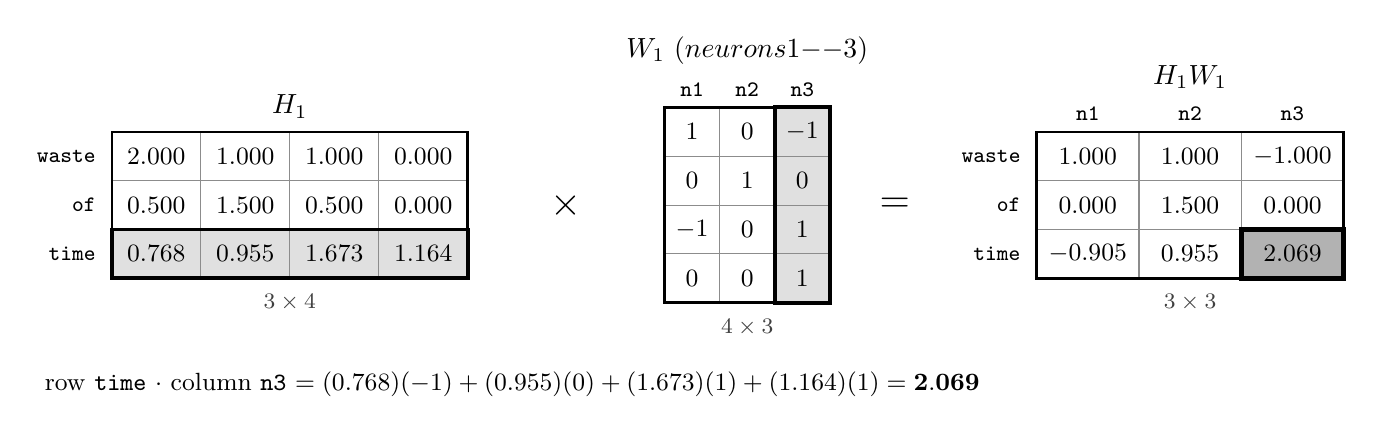
\begin{tikzpicture}
\draw[black!45, fill=white] (0.975,0.930) rectangle (2.105,0.310);
\node[font=\small, text=black] at (1.540,0.620) {$2.000$};
\draw[black!45, fill=white] (2.105,0.930) rectangle (3.235,0.310);
\node[font=\small, text=black] at (2.670,0.620) {$1.000$};
\draw[black!45, fill=white] (3.235,0.930) rectangle (4.365,0.310);
\node[font=\small, text=black] at (3.800,0.620) {$1.000$};
\draw[black!45, fill=white] (4.365,0.930) rectangle (5.495,0.310);
\node[font=\small, text=black] at (4.930,0.620) {$0.000$};
\draw[black!45, fill=white] (0.975,0.310) rectangle (2.105,-0.310);
\node[font=\small, text=black] at (1.540,-0.000) {$0.500$};
\draw[black!45, fill=white] (2.105,0.310) rectangle (3.235,-0.310);
\node[font=\small, text=black] at (2.670,-0.000) {$1.500$};
\draw[black!45, fill=white] (3.235,0.310) rectangle (4.365,-0.310);
\node[font=\small, text=black] at (3.800,-0.000) {$0.500$};
\draw[black!45, fill=white] (4.365,0.310) rectangle (5.495,-0.310);
\node[font=\small, text=black] at (4.930,-0.000) {$0.000$};
\draw[black!45, fill=black!12] (0.975,-0.310) rectangle (2.105,-0.930);
\node[font=\small, text=black] at (1.540,-0.620) {$0.768$};
\draw[black!45, fill=black!12] (2.105,-0.310) rectangle (3.235,-0.930);
\node[font=\small, text=black] at (2.670,-0.620) {$0.955$};
\draw[black!45, fill=black!12] (3.235,-0.310) rectangle (4.365,-0.930);
\node[font=\small, text=black] at (3.800,-0.620) {$1.673$};
\draw[black!45, fill=black!12] (4.365,-0.310) rectangle (5.495,-0.930);
\node[font=\small, text=black] at (4.930,-0.620) {$1.164$};
\draw[line width=1.4pt] (0.975,-0.310) rectangle (5.495,-0.930);
\draw[line width=0.9pt] (0.975,0.930) rectangle (5.495,-0.930);
\node[anchor=east, font=\footnotesize\ttfamily] at (0.895,0.620) {waste};
\node[anchor=east, font=\footnotesize\ttfamily] at (0.895,-0.000) {of};
\node[anchor=east, font=\footnotesize\ttfamily] at (0.895,-0.620) {time};
\node[anchor=south, font=\normalsize] at (3.235,0.980) {$H_1$};
\node[anchor=north, font=\footnotesize, text=black!75] at (3.235,-1.010) {$3\times4$};
\node[font=\Large] at (6.745,0) {$\times$};
\draw[black!45, fill=white] (7.995,1.240) rectangle (8.695,0.620);
\node[font=\small, text=black] at (8.345,0.930) {$1$};
\draw[black!45, fill=white] (8.695,1.240) rectangle (9.395,0.620);
\node[font=\small, text=black] at (9.045,0.930) {$0$};
\draw[black!45, fill=black!12] (9.395,1.240) rectangle (10.095,0.620);
\node[font=\small, text=black] at (9.745,0.930) {$-1$};
\draw[black!45, fill=white] (7.995,0.620) rectangle (8.695,0.000);
\node[font=\small, text=black] at (8.345,0.310) {$0$};
\draw[black!45, fill=white] (8.695,0.620) rectangle (9.395,0.000);
\node[font=\small, text=black] at (9.045,0.310) {$1$};
\draw[black!45, fill=black!12] (9.395,0.620) rectangle (10.095,0.000);
\node[font=\small, text=black] at (9.745,0.310) {$0$};
\draw[black!45, fill=white] (7.995,0.000) rectangle (8.695,-0.620);
\node[font=\small, text=black] at (8.345,-0.310) {$-1$};
\draw[black!45, fill=white] (8.695,0.000) rectangle (9.395,-0.620);
\node[font=\small, text=black] at (9.045,-0.310) {$0$};
\draw[black!45, fill=black!12] (9.395,0.000) rectangle (10.095,-0.620);
\node[font=\small, text=black] at (9.745,-0.310) {$1$};
\draw[black!45, fill=white] (7.995,-0.620) rectangle (8.695,-1.240);
\node[font=\small, text=black] at (8.345,-0.930) {$0$};
\draw[black!45, fill=white] (8.695,-0.620) rectangle (9.395,-1.240);
\node[font=\small, text=black] at (9.045,-0.930) {$0$};
\draw[black!45, fill=black!12] (9.395,-0.620) rectangle (10.095,-1.240);
\node[font=\small, text=black] at (9.745,-0.930) {$1$};
\draw[line width=1.4pt] (9.395,1.240) rectangle (10.095,-1.240);
\draw[line width=0.9pt] (7.995,1.240) rectangle (10.095,-1.240);
\node[anchor=south, font=\footnotesize\ttfamily] at (8.345,1.260) {n1};
\node[anchor=south, font=\footnotesize\ttfamily] at (9.045,1.260) {n2};
\node[anchor=south, font=\footnotesize\ttfamily] at (9.745,1.260) {n3};
\node[anchor=south, font=\normalsize] at (9.045,1.660) {$W_1\ (\text{neurons }1\text{--}3)$};
\node[anchor=north, font=\footnotesize, text=black!75] at (9.045,-1.320) {$4\times3$};
\node[font=\Large] at (10.920,0) {$=$};
\draw[black!45, fill=white] (12.720,0.930) rectangle (14.020,0.310);
\node[font=\small, text=black] at (13.370,0.620) {$1.000$};
\draw[black!45, fill=white] (14.020,0.930) rectangle (15.320,0.310);
\node[font=\small, text=black] at (14.670,0.620) {$1.000$};
\draw[black!45, fill=white] (15.320,0.930) rectangle (16.620,0.310);
\node[font=\small, text=black] at (15.970,0.620) {$-1.000$};
\draw[black!45, fill=white] (12.720,0.310) rectangle (14.020,-0.310);
\node[font=\small, text=black] at (13.370,-0.000) {$0.000$};
\draw[black!45, fill=white] (14.020,0.310) rectangle (15.320,-0.310);
\node[font=\small, text=black] at (14.670,-0.000) {$1.500$};
\draw[black!45, fill=white] (15.320,0.310) rectangle (16.620,-0.310);
\node[font=\small, text=black] at (15.970,-0.000) {$0.000$};
\draw[black!45, fill=white] (12.720,-0.310) rectangle (14.020,-0.930);
\node[font=\small, text=black] at (13.370,-0.620) {$-0.905$};
\draw[black!45, fill=white] (14.020,-0.310) rectangle (15.320,-0.930);
\node[font=\small, text=black] at (14.670,-0.620) {$0.955$};
\draw[black!45, fill=black!30] (15.320,-0.310) rectangle (16.620,-0.930);
\node[font=\small, text=black] at (15.970,-0.620) {$2.069$};
\draw[line width=1.6pt] (15.320,-0.310) rectangle (16.620,-0.930);
\draw[line width=0.9pt] (12.720,0.930) rectangle (16.620,-0.930);
\node[anchor=east, font=\footnotesize\ttfamily] at (12.640,0.620) {waste};
\node[anchor=east, font=\footnotesize\ttfamily] at (12.640,-0.000) {of};
\node[anchor=east, font=\footnotesize\ttfamily] at (12.640,-0.620) {time};
\node[anchor=south, font=\footnotesize\ttfamily] at (13.370,0.950) {n1};
\node[anchor=south, font=\footnotesize\ttfamily] at (14.670,0.950) {n2};
\node[anchor=south, font=\footnotesize\ttfamily] at (15.970,0.950) {n3};
\node[anchor=south, font=\normalsize] at (14.670,1.350) {$H_1W_1$};
\node[anchor=north, font=\footnotesize, text=black!75] at (14.670,-1.010) {$3\times3$};
\node[anchor=north west, font=\small, align=left] at (0,-1.990) {row \texttt{time} $\cdot$ column \texttt{n3} $= (0.768)(-1) + (0.955)(0) + (1.673)(1) + (1.164)(1) = \mathbf{2.069}$};
\end{tikzpicture}
}
\captionof{figure}{Step 1, the checks. Each column of $W_1$ is one neuron's key. The outlined row of $H_1$ (\tok{time}) meets neuron 3's key and gives the dark cell. Only the three neurons that are switched on are drawn; the other thirteen columns are zeros.}
\label{fig:ch5mlpone}
\end{center}

Second, add each neuron's threshold and let ReLU switch off everything negative
(Figure~\ref{fig:ch5mlptwo}).

\begin{center}
\fitwidthFourFive{% AUTO-GENERATED by code/figlib.py helpers -- do not edit
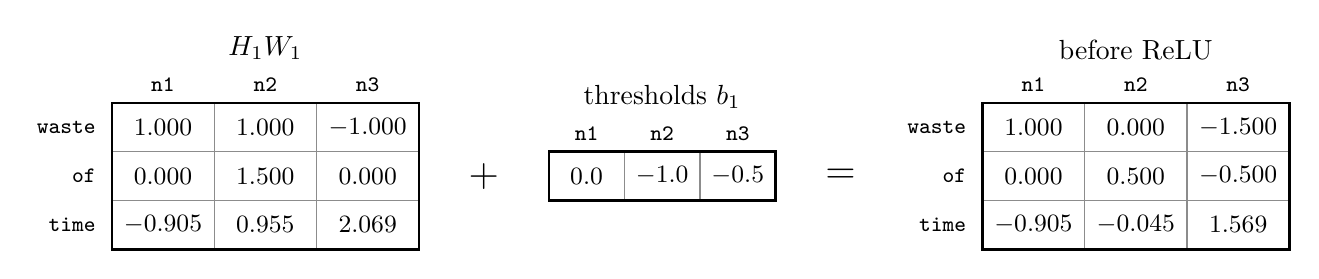
\begin{tikzpicture}
\draw[black!45, fill=white] (0.975,0.930) rectangle (2.275,0.310);
\node[font=\small, text=black] at (1.625,0.620) {$1.000$};
\draw[black!45, fill=white] (2.275,0.930) rectangle (3.575,0.310);
\node[font=\small, text=black] at (2.925,0.620) {$1.000$};
\draw[black!45, fill=white] (3.575,0.930) rectangle (4.875,0.310);
\node[font=\small, text=black] at (4.225,0.620) {$-1.000$};
\draw[black!45, fill=white] (0.975,0.310) rectangle (2.275,-0.310);
\node[font=\small, text=black] at (1.625,-0.000) {$0.000$};
\draw[black!45, fill=white] (2.275,0.310) rectangle (3.575,-0.310);
\node[font=\small, text=black] at (2.925,-0.000) {$1.500$};
\draw[black!45, fill=white] (3.575,0.310) rectangle (4.875,-0.310);
\node[font=\small, text=black] at (4.225,-0.000) {$0.000$};
\draw[black!45, fill=white] (0.975,-0.310) rectangle (2.275,-0.930);
\node[font=\small, text=black] at (1.625,-0.620) {$-0.905$};
\draw[black!45, fill=white] (2.275,-0.310) rectangle (3.575,-0.930);
\node[font=\small, text=black] at (2.925,-0.620) {$0.955$};
\draw[black!45, fill=white] (3.575,-0.310) rectangle (4.875,-0.930);
\node[font=\small, text=black] at (4.225,-0.620) {$2.069$};
\draw[line width=0.9pt] (0.975,0.930) rectangle (4.875,-0.930);
\node[anchor=east, font=\footnotesize\ttfamily] at (0.895,0.620) {waste};
\node[anchor=east, font=\footnotesize\ttfamily] at (0.895,-0.000) {of};
\node[anchor=east, font=\footnotesize\ttfamily] at (0.895,-0.620) {time};
\node[anchor=south, font=\footnotesize\ttfamily] at (1.625,0.950) {n1};
\node[anchor=south, font=\footnotesize\ttfamily] at (2.925,0.950) {n2};
\node[anchor=south, font=\footnotesize\ttfamily] at (4.225,0.950) {n3};
\node[anchor=south, font=\normalsize] at (2.925,1.350) {$H_1W_1$};
\node[font=\Large] at (5.700,0) {$+$};
\draw[black!45, fill=white] (6.525,0.310) rectangle (7.485,-0.310);
\node[font=\small, text=black] at (7.005,0.000) {$0.0$};
\draw[black!45, fill=white] (7.485,0.310) rectangle (8.445,-0.310);
\node[font=\small, text=black] at (7.965,0.000) {$-1.0$};
\draw[black!45, fill=white] (8.445,0.310) rectangle (9.405,-0.310);
\node[font=\small, text=black] at (8.925,0.000) {$-0.5$};
\draw[line width=0.9pt] (6.525,0.310) rectangle (9.405,-0.310);
\node[anchor=south, font=\footnotesize\ttfamily] at (7.005,0.330) {n1};
\node[anchor=south, font=\footnotesize\ttfamily] at (7.965,0.330) {n2};
\node[anchor=south, font=\footnotesize\ttfamily] at (8.925,0.330) {n3};
\node[anchor=south, font=\normalsize] at (7.965,0.730) {thresholds $\bm b_1$};
\node[font=\Large] at (10.230,0) {$=$};
\draw[black!45, fill=white] (12.030,0.930) rectangle (13.330,0.310);
\node[font=\small, text=black] at (12.680,0.620) {$1.000$};
\draw[black!45, fill=white] (13.330,0.930) rectangle (14.630,0.310);
\node[font=\small, text=black] at (13.980,0.620) {$0.000$};
\draw[black!45, fill=white] (14.630,0.930) rectangle (15.930,0.310);
\node[font=\small, text=black] at (15.280,0.620) {$-1.500$};
\draw[black!45, fill=white] (12.030,0.310) rectangle (13.330,-0.310);
\node[font=\small, text=black] at (12.680,-0.000) {$0.000$};
\draw[black!45, fill=white] (13.330,0.310) rectangle (14.630,-0.310);
\node[font=\small, text=black] at (13.980,-0.000) {$0.500$};
\draw[black!45, fill=white] (14.630,0.310) rectangle (15.930,-0.310);
\node[font=\small, text=black] at (15.280,-0.000) {$-0.500$};
\draw[black!45, fill=white] (12.030,-0.310) rectangle (13.330,-0.930);
\node[font=\small, text=black] at (12.680,-0.620) {$-0.905$};
\draw[black!45, fill=white] (13.330,-0.310) rectangle (14.630,-0.930);
\node[font=\small, text=black] at (13.980,-0.620) {$-0.045$};
\draw[black!45, fill=white] (14.630,-0.310) rectangle (15.930,-0.930);
\node[font=\small, text=black] at (15.280,-0.620) {$1.569$};
\draw[line width=0.9pt] (12.030,0.930) rectangle (15.930,-0.930);
\node[anchor=east, font=\footnotesize\ttfamily] at (11.950,0.620) {waste};
\node[anchor=east, font=\footnotesize\ttfamily] at (11.950,-0.000) {of};
\node[anchor=east, font=\footnotesize\ttfamily] at (11.950,-0.620) {time};
\node[anchor=south, font=\footnotesize\ttfamily] at (12.680,0.950) {n1};
\node[anchor=south, font=\footnotesize\ttfamily] at (13.980,0.950) {n2};
\node[anchor=south, font=\footnotesize\ttfamily] at (15.280,0.950) {n3};
\node[anchor=south, font=\normalsize] at (13.980,1.350) {before ReLU};
\end{tikzpicture}
\\[10pt]
\begin{tikzpicture}
\draw[black!45, fill=white] (0.975,0.930) rectangle (2.275,0.310);
\node[font=\small, text=black] at (1.625,0.620) {$1.000$};
\draw[black!45, fill=white] (2.275,0.930) rectangle (3.575,0.310);
\node[font=\small, text=black] at (2.925,0.620) {$0.000$};
\draw[black!45, fill=white] (3.575,0.930) rectangle (4.875,0.310);
\node[font=\small, text=black] at (4.225,0.620) {$-1.500$};
\draw[black!45, fill=white] (0.975,0.310) rectangle (2.275,-0.310);
\node[font=\small, text=black] at (1.625,-0.000) {$0.000$};
\draw[black!45, fill=white] (2.275,0.310) rectangle (3.575,-0.310);
\node[font=\small, text=black] at (2.925,-0.000) {$0.500$};
\draw[black!45, fill=white] (3.575,0.310) rectangle (4.875,-0.310);
\node[font=\small, text=black] at (4.225,-0.000) {$-0.500$};
\draw[black!45, fill=white] (0.975,-0.310) rectangle (2.275,-0.930);
\node[font=\small, text=black] at (1.625,-0.620) {$-0.905$};
\draw[black!45, fill=white] (2.275,-0.310) rectangle (3.575,-0.930);
\node[font=\small, text=black] at (2.925,-0.620) {$-0.045$};
\draw[black!45, fill=white] (3.575,-0.310) rectangle (4.875,-0.930);
\node[font=\small, text=black] at (4.225,-0.620) {$1.569$};
\draw[line width=0.9pt] (0.975,0.930) rectangle (4.875,-0.930);
\node[anchor=east, font=\footnotesize\ttfamily] at (0.895,0.620) {waste};
\node[anchor=east, font=\footnotesize\ttfamily] at (0.895,-0.000) {of};
\node[anchor=east, font=\footnotesize\ttfamily] at (0.895,-0.620) {time};
\node[anchor=south, font=\footnotesize\ttfamily] at (1.625,0.950) {n1};
\node[anchor=south, font=\footnotesize\ttfamily] at (2.925,0.950) {n2};
\node[anchor=south, font=\footnotesize\ttfamily] at (4.225,0.950) {n3};
\node[anchor=south, font=\normalsize] at (2.925,1.350) {before ReLU};
\node[font=\Large] at (8.420,0) {$\xrightarrow{\ \max(0,\,\cdot)\ }$};
\draw[black!45, fill=black!30] (12.940,0.930) rectangle (14.070,0.310);
\node[font=\small, text=black] at (13.505,0.620) {$1.000$};
\draw[black!45, fill=white] (14.070,0.930) rectangle (15.200,0.310);
\node[font=\small, text=black] at (14.635,0.620) {$0.000$};
\draw[black!45, fill=white] (15.200,0.930) rectangle (16.330,0.310);
\node[font=\small, text=black] at (15.765,0.620) {$0.000$};
\draw[black!45, fill=white] (12.940,0.310) rectangle (14.070,-0.310);
\node[font=\small, text=black] at (13.505,-0.000) {$0.000$};
\draw[black!45, fill=black!30] (14.070,0.310) rectangle (15.200,-0.310);
\node[font=\small, text=black] at (14.635,-0.000) {$0.500$};
\draw[black!45, fill=white] (15.200,0.310) rectangle (16.330,-0.310);
\node[font=\small, text=black] at (15.765,-0.000) {$0.000$};
\draw[black!45, fill=white] (12.940,-0.310) rectangle (14.070,-0.930);
\node[font=\small, text=black] at (13.505,-0.620) {$0.000$};
\draw[black!45, fill=white] (14.070,-0.310) rectangle (15.200,-0.930);
\node[font=\small, text=black] at (14.635,-0.620) {$0.000$};
\draw[black!45, fill=black!30] (15.200,-0.310) rectangle (16.330,-0.930);
\node[font=\small, text=black] at (15.765,-0.620) {$1.569$};
\draw[line width=1.6pt] (12.940,0.930) rectangle (14.070,0.310);
\draw[line width=1.6pt] (14.070,0.310) rectangle (15.200,-0.310);
\draw[line width=1.6pt] (15.200,-0.310) rectangle (16.330,-0.930);
\draw[line width=0.9pt] (12.940,0.930) rectangle (16.330,-0.930);
\node[anchor=east, font=\footnotesize\ttfamily] at (12.860,0.620) {waste};
\node[anchor=east, font=\footnotesize\ttfamily] at (12.860,-0.000) {of};
\node[anchor=east, font=\footnotesize\ttfamily] at (12.860,-0.620) {time};
\node[anchor=south, font=\footnotesize\ttfamily] at (13.505,0.950) {n1};
\node[anchor=south, font=\footnotesize\ttfamily] at (14.635,0.950) {n2};
\node[anchor=south, font=\footnotesize\ttfamily] at (15.765,0.950) {n3};
\node[anchor=south, font=\normalsize] at (14.635,1.350) {after ReLU: negatives become 0};
\end{tikzpicture}
}
\captionof{figure}{Step 2, thresholds and ReLU. Top: the thresholds are added to every row. Bottom: every negative number becomes 0. What survives sits on the diagonal (dark cells): neuron 1 fires on \tok{waste}, neuron 2 on \tok{of}, neuron 3 on \tok{time}.}
\label{fig:ch5mlptwo}
\end{center}

Third, each firing neuron writes its value, scaled by how strongly it fired (Figure~\ref{fig:ch5mlpthree}).

\begin{center}
\fitwidthFourFive{% AUTO-GENERATED by code/figlib.py helpers -- do not edit
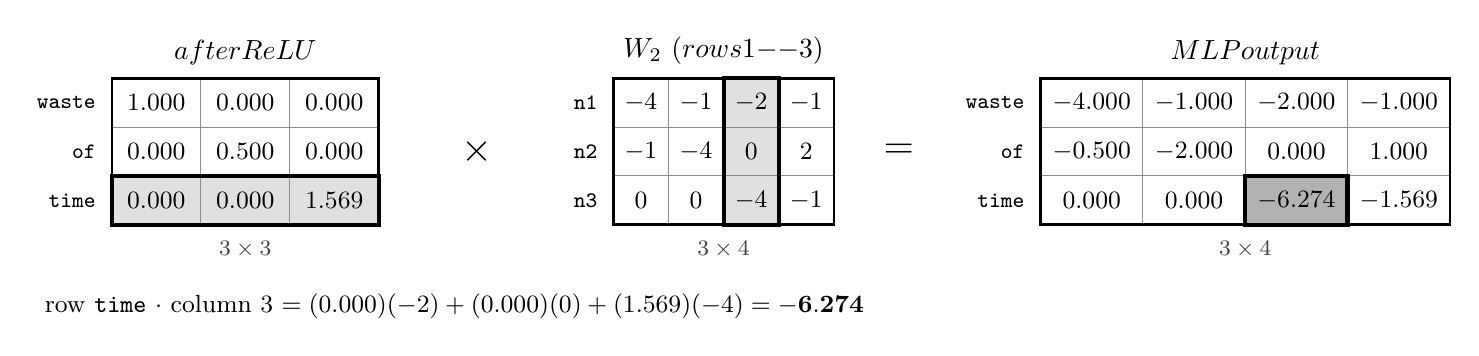
\begin{tikzpicture}
\draw[black!45, fill=white] (0.975,0.930) rectangle (2.105,0.310);
\node[font=\small, text=black] at (1.540,0.620) {$1.000$};
\draw[black!45, fill=white] (2.105,0.930) rectangle (3.235,0.310);
\node[font=\small, text=black] at (2.670,0.620) {$0.000$};
\draw[black!45, fill=white] (3.235,0.930) rectangle (4.365,0.310);
\node[font=\small, text=black] at (3.800,0.620) {$0.000$};
\draw[black!45, fill=white] (0.975,0.310) rectangle (2.105,-0.310);
\node[font=\small, text=black] at (1.540,-0.000) {$0.000$};
\draw[black!45, fill=white] (2.105,0.310) rectangle (3.235,-0.310);
\node[font=\small, text=black] at (2.670,-0.000) {$0.500$};
\draw[black!45, fill=white] (3.235,0.310) rectangle (4.365,-0.310);
\node[font=\small, text=black] at (3.800,-0.000) {$0.000$};
\draw[black!45, fill=black!12] (0.975,-0.310) rectangle (2.105,-0.930);
\node[font=\small, text=black] at (1.540,-0.620) {$0.000$};
\draw[black!45, fill=black!12] (2.105,-0.310) rectangle (3.235,-0.930);
\node[font=\small, text=black] at (2.670,-0.620) {$0.000$};
\draw[black!45, fill=black!12] (3.235,-0.310) rectangle (4.365,-0.930);
\node[font=\small, text=black] at (3.800,-0.620) {$1.569$};
\draw[line width=1.4pt] (0.975,-0.310) rectangle (4.365,-0.930);
\draw[line width=0.9pt] (0.975,0.930) rectangle (4.365,-0.930);
\node[anchor=east, font=\footnotesize\ttfamily] at (0.895,0.620) {waste};
\node[anchor=east, font=\footnotesize\ttfamily] at (0.895,-0.000) {of};
\node[anchor=east, font=\footnotesize\ttfamily] at (0.895,-0.620) {time};
\node[anchor=south, font=\normalsize] at (2.670,0.980) {$\text{after ReLU}$};
\node[anchor=north, font=\footnotesize, text=black!75] at (2.670,-1.010) {$3\times3$};
\node[font=\Large] at (5.615,0) {$\times$};
\draw[black!45, fill=white] (7.345,0.930) rectangle (8.045,0.310);
\node[font=\small, text=black] at (7.695,0.620) {$-4$};
\draw[black!45, fill=white] (8.045,0.930) rectangle (8.745,0.310);
\node[font=\small, text=black] at (8.395,0.620) {$-1$};
\draw[black!45, fill=black!12] (8.745,0.930) rectangle (9.445,0.310);
\node[font=\small, text=black] at (9.095,0.620) {$-2$};
\draw[black!45, fill=white] (9.445,0.930) rectangle (10.145,0.310);
\node[font=\small, text=black] at (9.795,0.620) {$-1$};
\draw[black!45, fill=white] (7.345,0.310) rectangle (8.045,-0.310);
\node[font=\small, text=black] at (7.695,-0.000) {$-1$};
\draw[black!45, fill=white] (8.045,0.310) rectangle (8.745,-0.310);
\node[font=\small, text=black] at (8.395,-0.000) {$-4$};
\draw[black!45, fill=black!12] (8.745,0.310) rectangle (9.445,-0.310);
\node[font=\small, text=black] at (9.095,-0.000) {$0$};
\draw[black!45, fill=white] (9.445,0.310) rectangle (10.145,-0.310);
\node[font=\small, text=black] at (9.795,-0.000) {$2$};
\draw[black!45, fill=white] (7.345,-0.310) rectangle (8.045,-0.930);
\node[font=\small, text=black] at (7.695,-0.620) {$0$};
\draw[black!45, fill=white] (8.045,-0.310) rectangle (8.745,-0.930);
\node[font=\small, text=black] at (8.395,-0.620) {$0$};
\draw[black!45, fill=black!12] (8.745,-0.310) rectangle (9.445,-0.930);
\node[font=\small, text=black] at (9.095,-0.620) {$-4$};
\draw[black!45, fill=white] (9.445,-0.310) rectangle (10.145,-0.930);
\node[font=\small, text=black] at (9.795,-0.620) {$-1$};
\draw[line width=1.4pt] (8.745,0.930) rectangle (9.445,-0.930);
\draw[line width=0.9pt] (7.345,0.930) rectangle (10.145,-0.930);
\node[anchor=east, font=\footnotesize\ttfamily] at (7.265,0.620) {n1};
\node[anchor=east, font=\footnotesize\ttfamily] at (7.265,-0.000) {n2};
\node[anchor=east, font=\footnotesize\ttfamily] at (7.265,-0.620) {n3};
\node[anchor=south, font=\normalsize] at (8.745,0.980) {$W_2\ (\text{rows }1\text{--}3)$};
\node[anchor=north, font=\footnotesize, text=black!75] at (8.745,-1.010) {$3\times4$};
\node[font=\Large] at (10.970,0) {$=$};
\draw[black!45, fill=white] (12.770,0.930) rectangle (14.070,0.310);
\node[font=\small, text=black] at (13.420,0.620) {$-4.000$};
\draw[black!45, fill=white] (14.070,0.930) rectangle (15.370,0.310);
\node[font=\small, text=black] at (14.720,0.620) {$-1.000$};
\draw[black!45, fill=white] (15.370,0.930) rectangle (16.670,0.310);
\node[font=\small, text=black] at (16.020,0.620) {$-2.000$};
\draw[black!45, fill=white] (16.670,0.930) rectangle (17.970,0.310);
\node[font=\small, text=black] at (17.320,0.620) {$-1.000$};
\draw[black!45, fill=white] (12.770,0.310) rectangle (14.070,-0.310);
\node[font=\small, text=black] at (13.420,-0.000) {$-0.500$};
\draw[black!45, fill=white] (14.070,0.310) rectangle (15.370,-0.310);
\node[font=\small, text=black] at (14.720,-0.000) {$-2.000$};
\draw[black!45, fill=white] (15.370,0.310) rectangle (16.670,-0.310);
\node[font=\small, text=black] at (16.020,-0.000) {$0.000$};
\draw[black!45, fill=white] (16.670,0.310) rectangle (17.970,-0.310);
\node[font=\small, text=black] at (17.320,-0.000) {$1.000$};
\draw[black!45, fill=white] (12.770,-0.310) rectangle (14.070,-0.930);
\node[font=\small, text=black] at (13.420,-0.620) {$0.000$};
\draw[black!45, fill=white] (14.070,-0.310) rectangle (15.370,-0.930);
\node[font=\small, text=black] at (14.720,-0.620) {$0.000$};
\draw[black!45, fill=black!30] (15.370,-0.310) rectangle (16.670,-0.930);
\node[font=\small, text=black] at (16.020,-0.620) {$-6.274$};
\draw[black!45, fill=white] (16.670,-0.310) rectangle (17.970,-0.930);
\node[font=\small, text=black] at (17.320,-0.620) {$-1.569$};
\draw[line width=1.6pt] (15.370,-0.310) rectangle (16.670,-0.930);
\draw[line width=0.9pt] (12.770,0.930) rectangle (17.970,-0.930);
\node[anchor=east, font=\footnotesize\ttfamily] at (12.690,0.620) {waste};
\node[anchor=east, font=\footnotesize\ttfamily] at (12.690,-0.000) {of};
\node[anchor=east, font=\footnotesize\ttfamily] at (12.690,-0.620) {time};
\node[anchor=south, font=\normalsize] at (15.370,0.980) {$\text{MLP output}$};
\node[anchor=north, font=\footnotesize, text=black!75] at (15.370,-1.010) {$3\times4$};
\node[anchor=north west, font=\small, align=left] at (0,-1.680) {row \texttt{time} $\cdot$ column 3 $= (0.000)(-2) + (0.000)(0) + (1.569)(-4) = \mathbf{-6.274}$};
\end{tikzpicture}
}
\captionof{figure}{Step 3, the values. The firing strengths times the rows of $W_2$. For \tok{time} only neuron 3 is non-zero, so its row of the output is $\nFiveNThreeTime$ times neuron 3's value.}
\label{fig:ch5mlpthree}
\end{center}

For \tok{time}, the MLP writes $\operatorname{MLP}(\bm{h}_{1,\text{time}}) = \nFiveMtime$.
Look at that value arrow: it mostly \emph{subtracts}. The arrow of \tok{time} is dominated by \tok{time}'s own
coordinates 3 and 4; neuron 3 removes them, and what is left is mostly the part attention brought in from
\tok{waste}. Writing by erasing is common: a pattern can say ``less of this'' as readily as ``more of that''.

\begin{breaks}
A checklist suggests each neuron has one clean meaning. In trained models, one neuron often responds to
several unrelated patterns, and one pattern is often spread across many neurons. The key--value reading is a
good first picture, not a complete one.
\end{breaks}

\Why Why work on each token alone? Attention has already done the talking: the arrow of \tok{time} now
carries what \tok{waste} and \tok{of} said. Thinking per token is cheap and fully parallel, because every row
is handled the same way at the same time. Why make the middle layer wider, $4d$? A wider middle means more
patterns to check, so a wider middle layer holds more keys. Why ReLU? It is the simplest function that can switch a pattern off. GPT-2 uses a
smooth cousin, GELU (Hendrycks and Gimpel, 2016), and Qwen uses a gated version, SwiGLU (Shazeer, 2020),
which multiplies two keys' answers together; Chapter 10 shows it on the real model.

\begin{wrongidea}{5.3}
\emph{The MLP is where tokens exchange information.} It comes right after attention, and it holds most of the
block's weights, so it is tempting to think it does the mixing. It does not: every row is processed alone.
It does not need to look back at the other tokens, because attention already carried the other tokens' information into this token's arrow.
\end{wrongidea}

\begin{checkq}
In the toy, change the arrow of \tok{waste} to anything you like, but leave $\bm{h}_{1}$ of \tok{time}
unchanged. What happens to the MLP's output for \tok{time}?
\begin{options}
\item It changes, because the MLP reads all three tokens.
\item It stays the same, because the MLP reads only the row it is working on.
\item It becomes zero, because \tok{waste}'s neuron stops firing.
\item It depends on the attention shares of \tok{waste}.
\end{options}
\end{checkq}

\Summary{The MLP checks each token's arrow, on its own, against a list of learned patterns and writes what the
firing patterns say.}

%---------------------------------------------------------------------
\subsection*{5.5\quad The residual stream: add, never overwrite}

There is one more piece, and it is the simplest. After attention, we did not \emph{replace} the arrow of
\tok{time} with $\bm{o}_{\text{time}}$. We \emph{added}:
\[
\bm{h}_1 = \bm{x} + \operatorname{Attn}(\bm{x}), \qquad \bm{h}_2 = \bm{h}_1 + \operatorname{MLP}(\bm{h}_1).
\]

\Picture A notebook is passed down a row of desks. Each desk reads the page and adds a note in the margin. No
desk tears the page out. Whoever reads the notebook at the end sees the original text and every note.

\Exactly For \tok{time}, the two additions are entry by entry (Figure~\ref{fig:ch5residual}).

\begin{center}
\fitwidthFourFive{% AUTO-GENERATED by code/figlib.py helpers -- do not edit
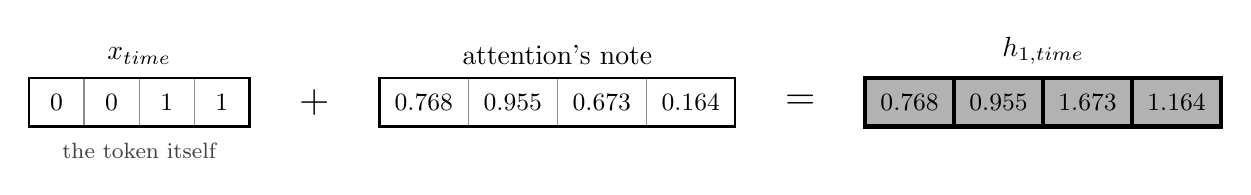
\begin{tikzpicture}
\draw[black!45, fill=white] (0.000,0.310) rectangle (0.700,-0.310);
\node[font=\small, text=black] at (0.350,0.000) {$0$};
\draw[black!45, fill=white] (0.700,0.310) rectangle (1.400,-0.310);
\node[font=\small, text=black] at (1.050,0.000) {$0$};
\draw[black!45, fill=white] (1.400,0.310) rectangle (2.100,-0.310);
\node[font=\small, text=black] at (1.750,0.000) {$1$};
\draw[black!45, fill=white] (2.100,0.310) rectangle (2.800,-0.310);
\node[font=\small, text=black] at (2.450,0.000) {$1$};
\draw[line width=0.9pt] (0.000,0.310) rectangle (2.800,-0.310);
\node[anchor=south, font=\normalsize] at (1.400,0.360) {$\bm x_{\text{time}}$};
\node[anchor=north, font=\footnotesize, text=black!75] at (1.400,-0.390) {the token itself};
\node[font=\Large] at (3.625,0) {$+$};
\draw[black!45, fill=white] (4.450,0.310) rectangle (5.580,-0.310);
\node[font=\small, text=black] at (5.015,0.000) {$0.768$};
\draw[black!45, fill=white] (5.580,0.310) rectangle (6.710,-0.310);
\node[font=\small, text=black] at (6.145,0.000) {$0.955$};
\draw[black!45, fill=white] (6.710,0.310) rectangle (7.840,-0.310);
\node[font=\small, text=black] at (7.275,0.000) {$0.673$};
\draw[black!45, fill=white] (7.840,0.310) rectangle (8.970,-0.310);
\node[font=\small, text=black] at (8.405,0.000) {$0.164$};
\draw[line width=0.9pt] (4.450,0.310) rectangle (8.970,-0.310);
\node[anchor=south, font=\normalsize] at (6.710,0.360) {attention's note};
\node[font=\Large] at (9.795,0) {$=$};
\draw[black!45, fill=black!30] (10.620,0.310) rectangle (11.750,-0.310);
\node[font=\small, text=black] at (11.185,0.000) {$0.768$};
\draw[black!45, fill=black!30] (11.750,0.310) rectangle (12.880,-0.310);
\node[font=\small, text=black] at (12.315,0.000) {$0.955$};
\draw[black!45, fill=black!30] (12.880,0.310) rectangle (14.010,-0.310);
\node[font=\small, text=black] at (13.445,0.000) {$1.673$};
\draw[black!45, fill=black!30] (14.010,0.310) rectangle (15.140,-0.310);
\node[font=\small, text=black] at (14.575,0.000) {$1.164$};
\draw[line width=1.6pt] (10.620,0.310) rectangle (11.750,-0.310);
\draw[line width=1.6pt] (11.750,0.310) rectangle (12.880,-0.310);
\draw[line width=1.6pt] (12.880,0.310) rectangle (14.010,-0.310);
\draw[line width=1.6pt] (14.010,0.310) rectangle (15.140,-0.310);
\draw[line width=0.9pt] (10.620,0.310) rectangle (15.140,-0.310);
\node[anchor=south, font=\normalsize] at (12.880,0.360) {$\bm h_{1,\text{time}}$};
\end{tikzpicture}
\\[10pt]
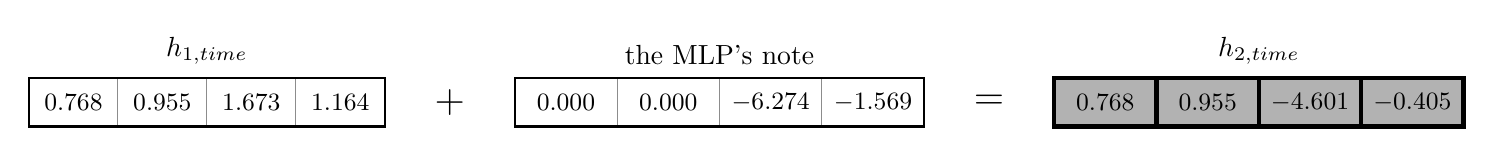
\begin{tikzpicture}
\draw[black!45, fill=white] (0.000,0.310) rectangle (1.130,-0.310);
\node[font=\small, text=black] at (0.565,0.000) {$0.768$};
\draw[black!45, fill=white] (1.130,0.310) rectangle (2.260,-0.310);
\node[font=\small, text=black] at (1.695,0.000) {$0.955$};
\draw[black!45, fill=white] (2.260,0.310) rectangle (3.390,-0.310);
\node[font=\small, text=black] at (2.825,0.000) {$1.673$};
\draw[black!45, fill=white] (3.390,0.310) rectangle (4.520,-0.310);
\node[font=\small, text=black] at (3.955,0.000) {$1.164$};
\draw[line width=0.9pt] (0.000,0.310) rectangle (4.520,-0.310);
\node[anchor=south, font=\normalsize] at (2.260,0.360) {$\bm h_{1,\text{time}}$};
\node[font=\Large] at (5.345,0) {$+$};
\draw[black!45, fill=white] (6.170,0.310) rectangle (7.470,-0.310);
\node[font=\small, text=black] at (6.820,0.000) {$0.000$};
\draw[black!45, fill=white] (7.470,0.310) rectangle (8.770,-0.310);
\node[font=\small, text=black] at (8.120,0.000) {$0.000$};
\draw[black!45, fill=white] (8.770,0.310) rectangle (10.070,-0.310);
\node[font=\small, text=black] at (9.420,0.000) {$-6.274$};
\draw[black!45, fill=white] (10.070,0.310) rectangle (11.370,-0.310);
\node[font=\small, text=black] at (10.720,0.000) {$-1.569$};
\draw[line width=0.9pt] (6.170,0.310) rectangle (11.370,-0.310);
\node[anchor=south, font=\normalsize] at (8.770,0.360) {the MLP's note};
\node[font=\Large] at (12.195,0) {$=$};
\draw[black!45, fill=black!30] (13.020,0.310) rectangle (14.320,-0.310);
\node[font=\small, text=black] at (13.670,0.000) {$0.768$};
\draw[black!45, fill=black!30] (14.320,0.310) rectangle (15.620,-0.310);
\node[font=\small, text=black] at (14.970,0.000) {$0.955$};
\draw[black!45, fill=black!30] (15.620,0.310) rectangle (16.920,-0.310);
\node[font=\small, text=black] at (16.270,0.000) {$-4.601$};
\draw[black!45, fill=black!30] (16.920,0.310) rectangle (18.220,-0.310);
\node[font=\small, text=black] at (17.570,0.000) {$-0.405$};
\draw[line width=1.6pt] (13.020,0.310) rectangle (14.320,-0.310);
\draw[line width=1.6pt] (14.320,0.310) rectangle (15.620,-0.310);
\draw[line width=1.6pt] (15.620,0.310) rectangle (16.920,-0.310);
\draw[line width=1.6pt] (16.920,0.310) rectangle (18.220,-0.310);
\draw[line width=0.9pt] (13.020,0.310) rectangle (18.220,-0.310);
\node[anchor=south, font=\normalsize] at (15.620,0.360) {$\bm h_{2,\text{time}}$};
\end{tikzpicture}
}
\captionof{figure}{The residual stream for \tok{time}. Top: the token's own arrow plus attention's note gives $\bm h_1$. Bottom: $\bm h_1$ plus the MLP's note gives $\bm h_2$. Nothing is replaced; each layer adds.}
\label{fig:ch5residual}
\end{center}

For the whole sentence, $H_2=\nFiveHtwo$.

The same block runs on every sentence of a batch at once, with the same weights. Figure~\ref{fig:ch5batch}
stacks $H_1$ for our two customer replies, the $B\times T\times d$ block of Chapter 3, \S3.9.

\begin{center}
\fitwidthFourFive{% AUTO-GENERATED by code/figlib.py helpers -- do not edit
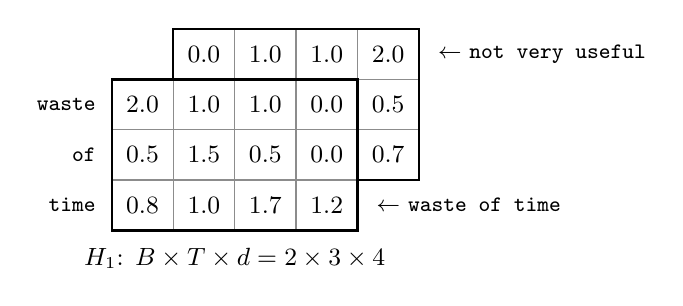
\begin{tikzpicture}
\fill[white] (0.780,0.640) rectangle (3.900,-1.279);
\draw[black!45, fill=white] (0.780,0.640) rectangle (1.560,0.000);
\node[font=\small, text=black] at (1.170,0.320) {$0.0$};
\draw[black!45, fill=white] (1.560,0.640) rectangle (2.340,0.000);
\node[font=\small, text=black] at (1.950,0.320) {$1.0$};
\draw[black!45, fill=white] (2.340,0.640) rectangle (3.120,0.000);
\node[font=\small, text=black] at (2.730,0.320) {$1.0$};
\draw[black!45, fill=white] (3.120,0.640) rectangle (3.900,0.000);
\node[font=\small, text=black] at (3.510,0.320) {$2.0$};
\draw[black!45, fill=white] (0.780,0.000) rectangle (1.560,-0.640);
\node[font=\small, text=black] at (1.170,-0.320) {$1.5$};
\draw[black!45, fill=white] (1.560,0.000) rectangle (2.340,-0.640);
\node[font=\small, text=black] at (1.950,-0.320) {$0.0$};
\draw[black!45, fill=white] (2.340,0.000) rectangle (3.120,-0.640);
\node[font=\small, text=black] at (2.730,-0.320) {$0.5$};
\draw[black!45, fill=white] (3.120,0.000) rectangle (3.900,-0.640);
\node[font=\small, text=black] at (3.510,-0.320) {$0.5$};
\draw[black!45, fill=white] (0.780,-0.640) rectangle (1.560,-1.279);
\node[font=\small, text=black] at (1.170,-0.959) {$0.4$};
\draw[black!45, fill=white] (1.560,-0.640) rectangle (2.340,-1.279);
\node[font=\small, text=black] at (1.950,-0.959) {$0.4$};
\draw[black!45, fill=white] (2.340,-0.640) rectangle (3.120,-1.279);
\node[font=\small, text=black] at (2.730,-0.959) {$1.7$};
\draw[black!45, fill=white] (3.120,-0.640) rectangle (3.900,-1.279);
\node[font=\small, text=black] at (3.510,-0.959) {$0.7$};
\draw[line width=0.9pt] (0.780,0.640) rectangle (3.900,-1.279);
\node[anchor=west, font=\footnotesize] at (4.020,0.320) {$\leftarrow$ \texttt{not very useful}};
\fill[white] (0.000,0.000) rectangle (3.120,-1.919);
\draw[black!45, fill=white] (0.000,0.000) rectangle (0.780,-0.640);
\node[font=\small, text=black] at (0.390,-0.320) {$2.0$};
\draw[black!45, fill=white] (0.780,0.000) rectangle (1.560,-0.640);
\node[font=\small, text=black] at (1.170,-0.320) {$1.0$};
\draw[black!45, fill=white] (1.560,0.000) rectangle (2.340,-0.640);
\node[font=\small, text=black] at (1.950,-0.320) {$1.0$};
\draw[black!45, fill=white] (2.340,0.000) rectangle (3.120,-0.640);
\node[font=\small, text=black] at (2.730,-0.320) {$0.0$};
\draw[black!45, fill=white] (0.000,-0.640) rectangle (0.780,-1.279);
\node[font=\small, text=black] at (0.390,-0.959) {$0.5$};
\draw[black!45, fill=white] (0.780,-0.640) rectangle (1.560,-1.279);
\node[font=\small, text=black] at (1.170,-0.959) {$1.5$};
\draw[black!45, fill=white] (1.560,-0.640) rectangle (2.340,-1.279);
\node[font=\small, text=black] at (1.950,-0.959) {$0.5$};
\draw[black!45, fill=white] (2.340,-0.640) rectangle (3.120,-1.279);
\node[font=\small, text=black] at (2.730,-0.959) {$0.0$};
\draw[black!45, fill=white] (0.000,-1.279) rectangle (0.780,-1.919);
\node[font=\small, text=black] at (0.390,-1.599) {$0.8$};
\draw[black!45, fill=white] (0.780,-1.279) rectangle (1.560,-1.919);
\node[font=\small, text=black] at (1.170,-1.599) {$1.0$};
\draw[black!45, fill=white] (1.560,-1.279) rectangle (2.340,-1.919);
\node[font=\small, text=black] at (1.950,-1.599) {$1.7$};
\draw[black!45, fill=white] (2.340,-1.279) rectangle (3.120,-1.919);
\node[font=\small, text=black] at (2.730,-1.599) {$1.2$};
\draw[line width=0.9pt] (0.000,0.000) rectangle (3.120,-1.919);
\node[anchor=east, font=\footnotesize\ttfamily] at (-0.080,-0.320) {waste};
\node[anchor=east, font=\footnotesize\ttfamily] at (-0.080,-0.959) {of};
\node[anchor=east, font=\footnotesize\ttfamily] at (-0.080,-1.599) {time};
\node[anchor=west, font=\footnotesize] at (3.240,-1.599) {$\leftarrow$ \texttt{waste of time}};
\node[anchor=north, font=\small] at (1.560,-2.019) {$H_1$: $B\times T\times d = 2\times3\times4$};
\end{tikzpicture}
}
\captionof{figure}{$H_1$ for a batch of two sentences (rounded to one decimal). The front sheet is \tok{waste of time}; the sheet behind is \tok{not very useful}. Every number in both sheets was made by the same heads and the same $W_O$.}
\label{fig:ch5batch}
\end{center}


Now read each row's guess for the next token, using the method Chapter 7 develops: compare the row with every
token's arrow by dot product and pick the largest. Row 1 picks \tok{\nFivePredWaste}, row 2 picks
\tok{\nFivePredOf}, row 3 picks \tok{\nFivePredTime} (score \nFiveLogitSorry, ahead of \tok{\nFiveTopTwoTime} at
\nFiveTopTwoTimeLogit). One pass, three positions, three correct next tokens: the $B\times T$ predictions of
\S1.9 on a real, if tiny, example.

\Predict What happens if we remove the residual additions, so that $\bm{h}_1=\operatorname{Attn}(\bm{x})$ and
$\bm{h}_2=\operatorname{MLP}(\bm{h}_1)$? Will the guesses survive?

\Sanity They do not. Without the additions the three rows guess \nFiveNoResPreds. Without the MLP but with the
additions, \tok{time} guesses \tok{\nFiveNoMlpPredTime}. Every piece is needed.

\paragraph{Deeper stacks.} A real model repeats the block many times. To see what the additions do over depth,
we stacked untrained blocks of a realistic shape ($d=\nFiveRbD$, \nFiveRbH\ heads, $d_{\text{ff}}=\nFiveRbDff$),
fed \nFiveRbSeqs\ random sentences of \nFiveRbT\ tokens from a vocabulary of \nFiveRbV, and asked after each
layer: can we still tell which token each position started as, by finding the nearest token arrow?

\begin{center}
\begin{tikzpicture}
\begin{axis}[width=10cm, height=5cm, xlabel={layers stacked}, ylabel={\% positions that know their token},
  ymin=-5, ymax=105, xmin=0, xmax=12, xtick={0,2,...,12}, axis lines*=left,
  tick label style={font=\small}, label style={font=\small}, legend style={font=\small, at={(0.5,-0.32)}, anchor=north, draw=none}, legend columns=2]
\addplot[thick, black, mark=*, mark size=1.4pt] table[x=L, y expr=100*\thisrow{res}] {data_ch5/identity.dat};
\addplot[thick, black!65, dashed, mark=square*, mark size=1.4pt] table[x=L, y expr=100*\thisrow{nores}] {data_ch5/identity.dat};
\legend{with residual additions, without residual additions}
\end{axis}
\end{tikzpicture}
\captionof{figure}{Untrained random blocks, fixed seed. With the additions, \nFiveIdResFour\% of positions still know their
token after 4 layers and \nFiveIdResTwelve\% after 12. Without them, \nFiveIdNoResOne\% after one layer: chance
level is \nFiveChance\%.}
\end{center}

Without the additions, one layer is enough to lose almost every token's identity: each layer overwrites the
arrow instead of adding to it, so what the token was at the start is gone.

\begin{breaks}
A notebook is only written on, but the residual stream can also be \emph{corrected}: neuron 3 wrote negative
numbers to cancel part of what was there. Think of margin notes that can say ``ignore the line above''.
\end{breaks}

\Why Adding keeps a straight path from the input to the output, so the original token and every layer's
contribution stay readable at the end. Elhage and colleagues (2021) call this shared space the \emph{residual
stream}: every layer reads from it and writes into it. The idea of adding a layer's input to its output comes
from image networks, where He and colleagues (2016) used it to train networks with more than a hundred layers.

\begin{wrongidea}{5.4}
\emph{Each layer replaces a token's arrow with a new one.} Diagrams draw layers as boxes in a row, which
suggests a relay where each runner drops what came before. The figure above shows what that would cost.
Each layer \emph{adds} to the arrow instead.
\end{wrongidea}

\begin{checkq}
In the toy, $\bm{x}_{\text{time}}=(0,0,1,1)$ and attention's output is $\nFiveO$. What is $\bm{h}_1$ for
\tok{time}?
\begin{options}
\item $\nFiveO$, because attention replaces the arrow.
\item $\nFiveHoneTime$, because the two are added.
\item $(0,0,1,1)$, because attention only changes other tokens.
\item The average of the two arrows.
\end{options}
\end{checkq}

\begin{principle}{add, do not overwrite}
Systems that must stay correct over many steps keep the original and append changes: a bank keeps every
transaction rather than only the balance; a version-control history keeps every commit. An agent's memory
layer that rewrites a stored memory in place loses the evidence of what was first said; one that keeps the raw
episode and adds annotations can always be checked and corrected later. The residual stream makes the same
choice inside the model.
\end{principle}

\Summary{Every layer adds its contribution to the token's arrow, so the original and every layer's notes stay
readable all the way to the top.}

%---------------------------------------------------------------------
\subsection*{5.6\quad The whole block, and where its weights live}

Putting it together, one block (still without the normalisation of Chapter 6) is
\[
\bm{h}_1 = \bm{x} + \big[\operatorname{head}_1(\bm{x})\ \ \operatorname{head}_2(\bm{x})\big]W_O,\qquad
\bm{h}_2 = \bm{h}_1 + \max(0,\ \bm{h}_1W_1+\bm{b}_1)\,W_2 .
\]
Count the weights. Attention holds four $d\times d$ matrices' worth ($W_Q$, $W_K$, $W_V$ split across the heads,
plus $W_O$): $4d^2$. The MLP holds $d\times4d$ plus $4d\times d$: $8d^2$. So about two thirds of a block's
weights sit in the MLP. In the toy: \nFiveParamsAttn\ in attention and \nFiveParamsMlp\ in the MLP (including
its 16 thresholds).

\Summary{A block is talk (heads), think (MLP) and add (residual), and most of its weights are in the thinking.}

\begin{lookingback}
(1) In Chapter 3, why was it $QK^\top$ and not $QK$? (2) In Chapter 4, which of $\bm{q}$, $\bm{k}$, $\bm{v}$
does RoPE rotate, and which does it leave alone? (3) In Chapter 1, how many next-token predictions does one pass
make for a batch of $B$ sentences of $T$ tokens?
\end{lookingback}

\begin{exercise}
Compute head 2's shares and output for the token \tok{of} (row 2). Explain the shares using the query alone.
\end{exercise}
\begin{exercise}
GPT-2 small has $d=\nFiveGptD$ and $d_{\text{ff}}=\nFiveGptDff$. Ignoring biases, how many weights are in one
block's attention, in its MLP, and in total?
\end{exercise}
\begin{exercise}
Using $H_1$ from \S5.4, design a fourth neuron (a key with entries from $\{-1,0,1\}$ and a threshold) that fires
on \tok{of} and on no other row. Is it unique?
\end{exercise}
\begin{exercise}
In your own words, explain to someone who has never seen a transformer why stacking twelve blocks without the
residual additions would fail, using the figure in \S5.5.
\end{exercise}

\subsection*{Answers to Chapter 5}
\small
\textbf{Check yourself 5.1.} (b). The output is one weighted average; different pairs of messages can give the
same average (\S5.1). (a) is M5.2: one head cannot keep two messages apart. (c) goes too far: the average is
still information. (d) is wrong: \tok{time}'s own share here is 0.

\textbf{Check yourself 5.2.} (b). $64/8=8$ numbers per head, and 8 separate softmaxes instead of 2. (a) is
backwards. (c) is wrong: the total size of $W_Q$, $W_K$, $W_V$, $W_O$ stays $4d^2$. (d) is M5.1.

\textbf{Check yourself 5.3.} (b). The MLP reads one row at a time. (a) and (d) are M5.3: the other tokens reach
\tok{time} only through attention, which happened before. (c) mixes up two rows: neuron 1 firing on \tok{waste}
does not affect \tok{time}'s row.

\textbf{Check yourself 5.4.} (b). The residual addition: $(0,0,1,1)+\nFiveO$. (a) is M5.4. (c) is wrong:
attention writes into every token's arrow, including \tok{time}'s. (d) halves both, which no step does.

\textbf{Answer 5.2 (head 2, your turn).} $\bm{q}^{(2)}_{\text{time}}=\nFiveQtwo$. The keys are the
columns of $K^{(2)\top}$ below, one per token; only \tok{of}'s is non-zero. Query against keys:

\begin{center}
\fitwidthFourFive{% AUTO-GENERATED by code/figlib.py helpers -- do not edit
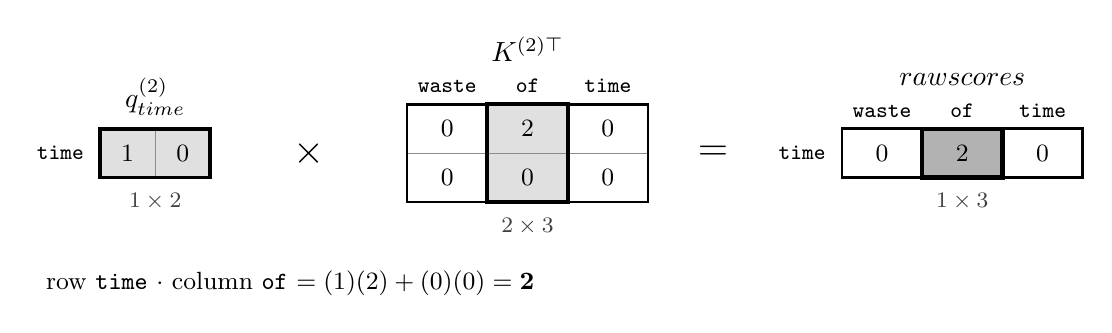
\begin{tikzpicture}
\draw[black!45, fill=black!12] (0.810,0.310) rectangle (1.510,-0.310);
\node[font=\small, text=black] at (1.160,0.000) {$1$};
\draw[black!45, fill=black!12] (1.510,0.310) rectangle (2.210,-0.310);
\node[font=\small, text=black] at (1.860,0.000) {$0$};
\draw[line width=1.4pt] (0.810,0.310) rectangle (2.210,-0.310);
\draw[line width=0.9pt] (0.810,0.310) rectangle (2.210,-0.310);
\node[anchor=east, font=\footnotesize\ttfamily] at (0.730,0.000) {time};
\node[anchor=south, font=\normalsize] at (1.510,0.360) {$\bm q^{(2)}_{\text{time}}$};
\node[anchor=north, font=\footnotesize, text=black!75] at (1.510,-0.390) {$1\times2$};
\node[font=\Large] at (3.460,0) {$\times$};
\draw[black!45, fill=white] (4.710,0.620) rectangle (5.730,0.000);
\node[font=\small, text=black] at (5.220,0.310) {$0$};
\draw[black!45, fill=black!12] (5.730,0.620) rectangle (6.750,0.000);
\node[font=\small, text=black] at (6.240,0.310) {$2$};
\draw[black!45, fill=white] (6.750,0.620) rectangle (7.770,0.000);
\node[font=\small, text=black] at (7.260,0.310) {$0$};
\draw[black!45, fill=white] (4.710,0.000) rectangle (5.730,-0.620);
\node[font=\small, text=black] at (5.220,-0.310) {$0$};
\draw[black!45, fill=black!12] (5.730,0.000) rectangle (6.750,-0.620);
\node[font=\small, text=black] at (6.240,-0.310) {$0$};
\draw[black!45, fill=white] (6.750,0.000) rectangle (7.770,-0.620);
\node[font=\small, text=black] at (7.260,-0.310) {$0$};
\draw[line width=1.4pt] (5.730,0.620) rectangle (6.750,-0.620);
\draw[line width=0.9pt] (4.710,0.620) rectangle (7.770,-0.620);
\node[anchor=south, font=\footnotesize\ttfamily] at (5.220,0.640) {waste};
\node[anchor=south, font=\footnotesize\ttfamily] at (6.240,0.640) {of};
\node[anchor=south, font=\footnotesize\ttfamily] at (7.260,0.640) {time};
\node[anchor=south, font=\normalsize] at (6.240,1.040) {$K^{(2)\top}$};
\node[anchor=north, font=\footnotesize, text=black!75] at (6.240,-0.700) {$2\times3$};
\node[font=\Large] at (8.595,0) {$=$};
\draw[black!45, fill=white] (10.230,0.310) rectangle (11.250,-0.310);
\node[font=\small, text=black] at (10.740,0.000) {$0$};
\draw[black!45, fill=black!30] (11.250,0.310) rectangle (12.270,-0.310);
\node[font=\small, text=black] at (11.760,0.000) {$2$};
\draw[black!45, fill=white] (12.270,0.310) rectangle (13.290,-0.310);
\node[font=\small, text=black] at (12.780,0.000) {$0$};
\draw[line width=1.6pt] (11.250,0.310) rectangle (12.270,-0.310);
\draw[line width=0.9pt] (10.230,0.310) rectangle (13.290,-0.310);
\node[anchor=east, font=\footnotesize\ttfamily] at (10.150,0.000) {time};
\node[anchor=south, font=\footnotesize\ttfamily] at (10.740,0.330) {waste};
\node[anchor=south, font=\footnotesize\ttfamily] at (11.760,0.330) {of};
\node[anchor=south, font=\footnotesize\ttfamily] at (12.780,0.330) {time};
\node[anchor=south, font=\normalsize] at (11.760,0.730) {$\text{raw scores}$};
\node[anchor=north, font=\footnotesize, text=black!75] at (11.760,-0.390) {$1\times3$};
\node[anchor=north west, font=\small, align=left] at (0,-1.370) {row \texttt{time} $\cdot$ column \texttt{of} $= (1)(2) + (0)(0) = \mathbf{2}$};
\end{tikzpicture}
}
\end{center}

\noindent Raw scores $\nFiveStwo$; scaled $\nFiveStwoScaled$; shares
$(\nFiveAtwoWaste, \nFiveAtwoOf, \nFiveAtwoTime)$.

\textbf{Looking back.} (1) $Q$ and $K$ are both $T\times d_k$; only $QK^\top$ pairs each query row with each key
row. (2) RoPE rotates queries and keys; values are left alone. (3) $B\times T$.

\textbf{Exercise 5.1.} $\bm{q}^{(2)}_{\text{of}}=\nFiveQtwoOf$: a query of all zeros scores every key 0, so the
shares are $\nFiveAtwoOfRow$ over \tok{waste} and \tok{of}, and the output is $\nFiveOtwoOfRow$. An empty question
gives the plain average, as in Chapter 3.

\textbf{Exercise 5.2.} Attention $4d^2=\nFiveGptAttn$; MLP $2\times d\times d_{\text{ff}}=\nFiveGptMlp$; total
\nFiveGptBlock. Chapter 10 checks this against the real model, biases and norms included.

\textbf{Exercise 5.3.} Neuron 2, key $(0,1,0,0)$ with threshold $-1$, already works: it gives $\nFiveNTwoOf$ on \tok{of}
and nothing elsewhere. Others work too, for example $(-1,1,0,0)$ with threshold $0$. It is not unique: many keys
separate the rows, which is one reason trained neurons are hard to name.

\textbf{Exercise 5.4.} Without the additions, each layer's output is all that reaches the next layer. After one
untrained layer only \nFiveIdNoResOne\% of positions can still be matched to their starting token, roughly chance;
with the additions, the original arrow travels up unchanged and later layers add to it.
\normalsize

\subsection*{What you now know}
\begin{itemize}
\item Why one head returns one blend, and why several narrower heads can ask several questions at the same cost.
\item How head outputs are concatenated and mixed by $W_O$.
\item How the MLP works on each token alone, as keys (patterns), thresholds and values.
\item Why every layer adds to the residual stream instead of replacing it, with measured numbers.
\item How one toy block predicts \tok{of}, \tok{time} and \tok{Sorry} at the three positions in a single pass.
\end{itemize}
